\documentclass[aspectratio=169,10pt]{beamer}


%%%%%%%%%%%%%%%%% Algunos paquetes especiales %%%%%%%%%%%%%%%%%
%\usepackage[spanish]{babel}
\usepackage[main=spanish,locale=US]{babel}
%\usepackage[T1]{fontenc}
\usepackage[utf8]{inputenc}
\usepackage{siunitx}
\sisetup{output-decimal-marker = {.}}
\usepackage{pgf-pie}
\usepackage{graphicx}
\usepackage{multicol}
\usepackage[utf8]{inputenc}
%\usepackage[latin1]{inputenc}
%\unaccentedoperators
\usepackage[nodayofweek,level]{datetime}
\usepackage{tikz}
\usepackage{pgfplots}
    %\pgfplotsset{compat=1.18}
\usetikzlibrary{positioning} 
\usepackage{pgfplotstable}
\usetikzlibrary{patterns, arrows.meta}
\usepgfplotslibrary{dateplot}
\usepackage{fancyhdr}
\usepackage{longtable}
\usepackage{graphicx}
\usepackage{threeparttablex}
\usepackage{rotating}
\usepackage{fontsize}
  \changefontsize[13.8pt]{12pt}
\usepackage{gensymb}
\usepackage{cancel}
\usepackage{multicol}
\usepackage{tabulary}
\usepackage{nccmath}
\usepackage{chemfig}
%\usepackage[hyphens]{url}
\usepackage{float}
\usepackage[
  labelfont=bf,
  singlelinecheck=false,
  indention=2.4cm,
  format=plain,
  parindent=1em,
  justification=centering
]{caption}
\usepackage{subcaption}
\usepackage{hyperref}
\usepackage{tikz}
\usepackage{array,ragged2e, tabularx}
\usepackage{tcolorbox}
\usepackage[export]{adjustbox}
\usepackage{microtype}
\usepackage{wasysym}
\usepackage{colortbl}
\usepackage{hhline}
\usepackage{lscape}
\usetikzlibrary{mindmap}
\usepackage{enumerate} 
\usepackage{enumitem} 
\usepackage{mathtools}
\usepackage{amssymb}
\usepackage{multirow}
\usepackage{etoolbox}
\usepackage{marvosym}
\usepackage[section]{placeins}
\usepackage{calc} 
\usepackage{newfloat}
\usepackage{lipsum}  
\usepackage{xcolor}  
\newcolumntype{P}[1]{>{\raggedRight}p{#1}}
\usepackage[style=authoryear, citestyle=authoryear]{biblatex}
\DeclareDelimFormat[nameyeardelim]{nameyeardelim}{\addspace} % Elimina la coma
%\usepackage[spanish]{babel}
%\usepackage[utf8]{inputenc}
\usepackage{graphicx}
\usepackage{amsmath}
\usepackage{booktabs}
\usepackage{xcolor}


\usetheme{Singapore}
\usecolortheme{orchid}

\setbeamertemplate{navigation symbols}{} % Sin íconos de navegación
\setbeamertemplate{footline}[page number] % Solo número de página en pie
\setbeamertemplate{headline}{} % Sin barra superior

% Información del título
\title{\Large El Laberinto Fiscal de Colombia}
\subtitle{Causas, Riesgos y Salidas a la Crisis Fiscal}
\author{Oliver Pardo}
\institute{Director del Centro Javeriano de Competitividad y Profesor Asociado de la Pontificia Universidad Javeriana.\\[0.12cm]
{\scriptsize\ttfamily javeriana.edu.co/centro-competitividad}\\[-0.02cm]
{\scriptsize\ttfamily oliverpardoeconomia.com}}
\date{Mayo de 2026}

\begin{document}

\begin{frame}{}
\centering
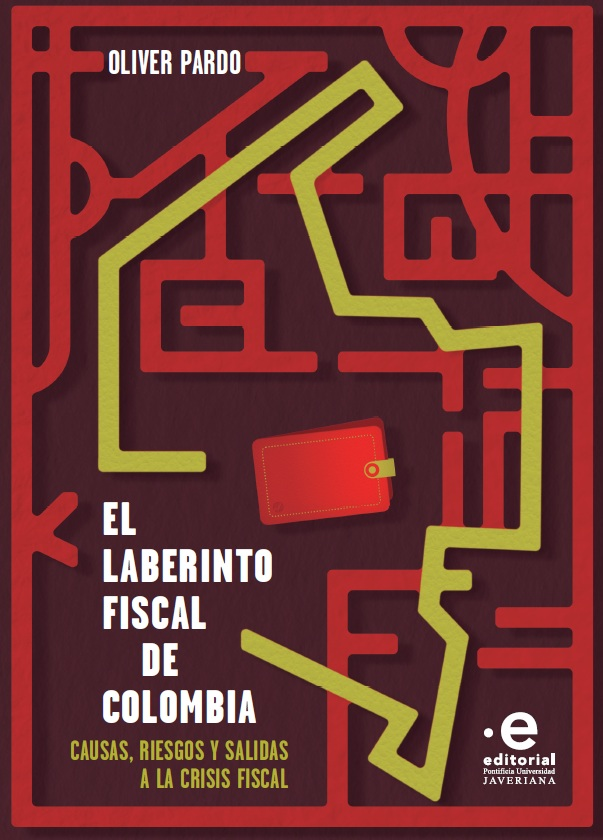
\includegraphics[scale=0.5]{graficas/Cover.jpg}
%
\includegraphics[scale=0.5]{graficas/QR.jpeg}
\end{frame}


\begin{frame}
    \titlepage
    \note{[Sources] Centro Javeriano de Competitividad: https://www.javeriana.edu.co/centro-competitividad. Página personal: https://oliverpardoeconomia.com/. Consultadas el 21 de agosto de 2026.}
\end{frame}

% Una sola vez al inicio: todas las secciones
\begin{frame}{Contenido}
  \tableofcontents
\end{frame}

% Al inicio de cada sección: todas visibles, actual resaltada
\AtBeginSection[]{
  \begin{frame}{Contenido}
    \tableofcontents[sectionstyle=show/shaded, subsectionstyle=show/show/shaded]
  \end{frame}
}
%\section{Presentación}
%\begin{frame}
    \frametitle{Objetivos del libro}  
    \begin{itemize}
        \item Presentar la evolución reciente de las finanzas públicas
        \item Dimensionar la magnitud de la problemática presente y futura 
        \item Proponer soluciones para recuperar la sostenibilidad fiscal
    \end{itemize}
\end{frame}

\begin{frame}
    \frametitle{Mensajes clave}  
\begin{block}{Reformas legales y constitucionales}
La magnitud del ajuste fiscal requerido desborda las capacidades del gobierno bajo el marco legal e institucional vigente, lo que hace indispensables reformas legales y constitucionales.
\end{block}
\begin{block}{El gasto público difícilmente podrá reducirse significativamente.}
Las reformas al gasto son necesarias, pero sus efectos se reflejarán más en la contención del crecimiento del gasto que en recortes significativos.
\end{block}
\begin{block}{Se necesita al menos una reforma tributaria, pero...}
Se requiere de un aumento significativo de los ingresos tributarios, lo cual necesita como prerequisito reflexionar sobre el fracaso de las reformas tributarias recientes.
\end{block}
\end{frame}

\begin{frame}{Metodología y fuentes}
\begin{itemize}
    \item Análisis centrado en el Gobierno Nacional Central (GNC).
    \item Cifras en \% del PIB. 0,1\% equivale a $\sim$\$1,8 billones en 2025.
    \item Datos oficiales ajustados para claridad y consistencia.
    \item Fuentes: MinHacienda, DIAN y CARF, principalmente.
    \item Material disponible en: \url{https://sites.google.com/site/oliverpardo/}
\end{itemize}
\end{frame}


\section{¿Qué tan profundo es el laberinto fiscal?}
\begin{frame}{¿Qué tan profundo es el laberinto fiscal?}
    \begin{itemize}
        \item Salir del laberinto fiscal enfrenta una paradoja:
        \begin{itemize}
            \item Por un lado, es necesario reconocer lo profundo del laberinto.
            \item Por otro lado, el pesimismo se puede convertir en una profecía autocumplida. 
        \end{itemize}
    \end{itemize}
\end{frame}

\begin{frame}{¿Qué tan profundo es el laberinto fiscal?}
    \begin{itemize}
        \item La consolidación fiscal en Colombia requerirá una combinación políticamente difícil de mayor recaudo, contención del gasto y una nueva regla fiscal.
        \item Si no se construye el consenso político necesario para ese ajuste, la corrección terminará siendo impuesta por restricciones de liquidez.
        \item En ese escenario, el ajuste se daría mediante recortes abruptos, congelamiento de apropiaciones, atrasos en pagos y, en un caso extremo, incumplimientos de obligaciones financieras.
    \end{itemize}
\end{frame}
\begin{frame}{¿Qué tan profundo es el laberinto fiscal?}
    \begin{itemize}
        \item El déficit primario alcanzó 3,5\% del PIB en 2025.
        \item Frenar el crecimiento de la deuda requerirá alcanzar un superávit primario cercano al 1,5\% del PIB.
        \item De inmediato queda claro que el ajuste fiscal deberá:
        \begin{itemize}
            \item Ser gradual.
            \item Incluir medidas tanto de ingresos como de gastos.
            \item Estar acompañados de políticas que aceleren el crecimiento económico.
        \end{itemize}
        \item Sin embargo, el paquete de medidas necesario para lograr la consolidación fiscal sumará \textbf{más} de 5\% del PIB. 
        \end{itemize}
\end{frame}


\section{¿Cómo aumentar los ingresos?}
\begin{frame}
  \frametitle{Ingresos tributarios del GNC}
  \vspace{0.05cm}
  {\centering\small\color{blue!70!black}Fuente: MHCP y cálculos propios\par}
  \vspace{-0.1cm}
  \begin{center}
    \scalebox{0.70}{
      \begin{tikzpicture}
      \begin{axis}[
          width=16.5cm,
          height=9.5cm,
          ylabel={\% PIB},
          xtick={1,...,24},
          xticklabels={2004,2005,2006,2007,2008,2009,2010,2011,2012,2013,2014,2015,2016,2017,2018,2019,2020,2021,2022,2023,2024,2025,2026,2027},
          x tick label style={rotate=90, anchor=east},
          ymin=11,
          ymax=17,
          grid=major,
          grid=both,
          grid style=dashed,
          minor y tick num=1,
          legend style={at={(0.05,0.9)}, anchor=north west},
          legend cell align={left},
          thick
      ]

%      % Ingreso Total
%      \addplot[
%          mark=square*,
%          dashed,
%          red
%      ] coordinates {
%          (1,13.2) (2,13.6) (3,14.8) (4,15.1) (5,15.8) (6,15.4) (7,13.8)
%          (8,15.2) (9,16.1) (10,16.8) (11,16.5) (12,16.1) (13,14.9) (14,15.7)
%          (15,15.1) (16,16.2) (17,15.3) (18,16.1) (19,16.2) (20,18.7) (21,16.5) (22,16.3)
%      };

      % Ingreso Tributario
      \addplot[
          mark=*,
          very thick,
          blue
      ] coordinates {
          (1,12.143374781333) (2,12.512922935182) (3,13.422519626341)
          (4,13.504136808694) (5,13.502896432021) (6,12.998278577445)
          (7,12.274640215080) (8,13.538733320074) (9,14.274306787792)
          (10,14.112999163893) (11,14.201344469556) (12,14.465553461687)
          (13,13.583123624578) (14,13.792707184015) (15,13.685807298757)
          (16,14.000802323615) (17,13.096318634224) (18,13.602505788695)
          (19,14.411093615786) (20,16.609633331004) (21,14.360250034683)
          (22,14.667199811906)
      };

      % Proyección MHCP 2026--2027, hoja 1.3 de Figuras.xlsx
      \addplot[
          color=blue,
          mark=*,
          very thick,
          densely dotted
      ] coordinates {
          (22,14.667199811906) (23,14.5) (24,14.0)
      };

      \node[anchor=south] at (axis cs:23,14.5) {\scriptsize 14,5};
      \node[anchor=north] at (axis cs:24,14.0) {\scriptsize 14,0};

      % Promedio 2012--2025 (Ingreso Tributario)
      \pgfmathsetmacro{\avgtrib}{14.204546109299}
      \addplot[
          red,
          dashed,
          thick
      ] coordinates {(9,\avgtrib) (22,\avgtrib)};

      \legend{Ingreso tributario, Proyección 2026--2027, Promedio 2012--2025}
      \end{axis}
      \end{tikzpicture}
    }
  \end{center}
  \note{[Sources] Figuras.xlsx, hoja 1.3, B1:Y1 y B3:Y4, versión del 17 de septiembre de 2026. Fuente indicada en el Excel: MHCP. Ingreso tributario del GNC, 2004--2027, en porcentaje del PIB. Las proyecciones para 2026 y 2027 son 14,5\% y 14,0\% del PIB, respectivamente. La línea discontinua conecta las proyecciones con el dato de 2025. Promedio aritmético de 2012--2025, calculado con los valores sin redondear de J3:W3: 14,204546109299\% del PIB.}
\end{frame}

\begin{frame}{Hipótesis sobre el estancamiento}
\begin{itemize}
    \item Tarifas por encima de las que maximizan el recaudo.
    \item Economía política de las reformas tributarias.
    \item Deficiencias administrativas de la DIAN.
\end{itemize}
\end{frame}
\begin{frame}{Aportes sobre el IBC: dependientes e independientes}
\begin{table}[h!]
\centering
\small
\begin{tabular}{|l|cc|cc|cc|cc|}
\hline
\multirow{2}{*}{\textbf{Aportes \textbackslash{} IBC}} & \multicolumn{2}{c}{\textbf{1 SMLMV}} & \multicolumn{2}{|c|}{\textbf{2 SMLMV}} & \multicolumn{2}{|c|}{\textbf{4 SMLMV}} & \multicolumn{2}{|c|}{\textbf{10 SMLMV}} \\
& \textbf{Dep.} & \textbf{Ind.} & \textbf{Dep.} & \textbf{Ind.} & \textbf{Dep.} & \textbf{Ind.} & \textbf{Dep.} & \textbf{Ind.} \\ \hline
Salud (Empresa)     & 0,0\  & 0,0\  & 0,0\  & 0,0\  & 0,0\  & 0,0\  & 8,5\  & 0,0\  \\
Salud (Trab.)  & 4,0\  & 12,5\ & 4,0\  & 12,5\ & 4,0\  & 12,5\ & 4,0\  & 12,5\ \\
Pensión (Empresa)   & 12,0\ & 0,0\  & 12,0\ & 0,0\  & 12,0\ & 0,0\  & 12,0\ & 0,0\  \\
Pensión (Trab.) & 4,0\  & 16,0\ & 4,0\  & 16,0\ & 4,0\  & 16,0\ & 4,0\  & 16,0\ \\
Riesgos Laborales        & 0,5\  & 0,5\  & 0,5\  & 0,5\  & 0,5\  & 0,5\  & 0,5\  & 0,5\  \\
Caja de C. F.     & 4,0\  & 2,0\  & 4,0\  & 2,0\  & 4,0\  & 2,0\  & 4,0\  & 2,0\  \\
SENA e ICBF               & 0,0\  & 0,0\  & 0,0\  & 0,0\  & 0,0\  & 0,0\  & 5,0\  & 0,0\  \\
Fondo solidaridad        & 0,0\  & 0,0\  & 0,0\  & 0,0\  & 1,0\  & 1,0\  & 1,0\  & 1,0\  \\ \hline
\textbf{Total}           & \textbf{24,5}\ & \textbf{31,0}\ & \textbf{24,5}\ & \textbf{31,0}\ & \textbf{25,5}\ & \textbf{32,0}\ & \textbf{39,0}\ & \textbf{36,0}\ \\ \hline
\end{tabular}
\vspace{0.1cm} 
\par \scriptsize{\textit{Nota: ARL corresponde a la tarifa mínima, redondeada a 0,5\%. Para independientes, la afiliación a caja de compensación (2\%) y, según la modalidad contractual, a ARL puede ser voluntaria.}}

\vspace{0.08cm}
\par \scriptsize{\textit{Fuente: elaboración propia con base en UGPP y el artículo 114-1 del Estatuto Tributario; colaboración de Mauricio Salazar.}}
\end{table}

\note{[Sources] UGPP, Seguridad social para trabajadores independientes: https://www.ugpp.gov.co/seguridad-social-trabajadores-independientes/. DIAN, artículo 114-1 del Estatuto Tributario: https://normograma.dian.gov.co/dian/compilacion/docs/estatuto_tributario.htm. Consultadas el 20 de agosto de 2026.}
\end{frame}

\begin{frame}{Beneficios en renta de personas jurídicas por actividad (2021)}
\begin{table}[h!]
    \centering
    \small
    \setlength{\tabcolsep}{4pt}
    \renewcommand{\arraystretch}{1.05}
    \begin{tabular}{@{}c p{0.62\textwidth} c@{}}
        \toprule
        & \textbf{Actividad económica} & \shortstack{\textbf{Gasto tributario}\\(\% del PIB)} \\
        \midrule
        1  & Transmisión de energía eléctrica & 0,13\% \\
        2  & Actividades de planes de seguridad social obligatoria & 0,11\% \\
        3  & Otras actividades del mercado de valores & 0,11\% \\
        4  & Banco central y bancos comerciales & 0,09\% \\
        5  & Distribución de energía eléctrica & 0,07\% \\
        6  & Extracción de petróleo crudo & 0,06\% \\
        7  & Actividades de administración empresarial & 0,06\% \\
        8  & Seguros de vida & 0,05\% \\
        9  & Producción de malta y cervezas & 0,03\% \\
        10 & Otras actividades de servicio financiero & 0,03\% \\
        \midrule
        & \textbf{Total} & \textbf{0,74\%} \\
        \bottomrule
    \end{tabular}
    \vspace{0.12cm}
    \par\scriptsize{\textit{Fuente: Cuadro 6.3 de El laberinto fiscal de Colombia, con base en Pardo et al. (2024).}}
\end{table}

\note{[Sources] Cuadro 6.3 de El laberinto fiscal de Colombia: https://www.laberintofiscal.co/capitulos/6-inevitables-como-la-muerte/\#table-6-3. Fuente original: Pardo, O.; Heredia, L.; Nieto, A.; y Millán, G. (2024), ``La tributación en impuesto sobre la renta por actividad económica en Colombia'', Coyuntura Económica, vol. 54. El total de 0,74\% del PIB corresponde a la suma de las diez actividades y coincide con la edición definitiva y la versión web.}
\end{frame}

\begin{frame}{Brecha tributaria}
\begin{itemize}
    \item Brecha tributaria = brecha de cumplimiento + brecha de política
    \item Brecha de cumplimiento (evasión) = 8,6\% del PIB.
    \item Brecha de política (gasto tributario) = 8,5\% del PIB.
    \item \textbf{Bajo el marco tributario de referencia, el GNC debería estar recaudando más del 30\% del PIB}
\end{itemize}
\end{frame}

\begin{frame}
\begin{table}[htbp]
\centering
\caption{Evasión por tipo de impuesto}
\label{tab:evasion_recaudo}
\large
\setlength{\tabcolsep}{7pt}
\renewcommand{\arraystretch}{1.22}
\begin{tabular}{lccc}
\toprule
Impuesto
& \shortstack{Recaudo\\(2025)\\\% del PIB}
& \shortstack{Evasión\\(2019)\\\% del PIB}
& \shortstack{Evasión\\(2019)\\\% del recaudo$^{*}$} \\
\midrule
IVA & 5,3 & \textbf{1,8} & 34\% \\
\shortstack[l]{Renta de personas\\jurídicas} & 6,0 & \textbf{5,7} & 95\% \\
\shortstack[l]{Renta de personas\\naturales} & 1,5 & \textbf{1,1} & 73\% \\
\bottomrule
\end{tabular}
\vspace{0.35cm}

\par\scriptsize{$^{*}$ Cociente entre la evasión estimada para 2019 y el recaudo de 2025. El porcentaje muestra un orden de magnitud y no una comparación para un mismo año.}

\vspace{0.12cm}
\par\scriptsize{\textit{Fuentes: Evasión con base en Lora et al. (2021). Recaudo con cálculos propios a partir del Balance del GNC del Ministerio de Hacienda.}}
\end{table}

\note{[Sources] Evasión: Lora et al. (2021), estimaciones para 2019. Recaudo: cálculos propios a partir del Balance del GNC del Ministerio de Hacienda, cifras para 2025. Los porcentajes del recaudo se calculan como evasión dividida por el recaudo de 2025.}

\end{frame}

\begin{frame}
\begin{table}[htbp]
\centering
\caption{Gasto tributario por tipo de impuesto}
\label{tab:gasto_tributario_recaudo}
\large
\setlength{\tabcolsep}{7pt}
\renewcommand{\arraystretch}{1.22}
\begin{tabular}{lccc}
\toprule
Impuesto
& \shortstack{Recaudo\\(2025)\\\% del PIB}
& \shortstack{Gasto tributario\\(2023)\\\% del PIB}
& \shortstack{Gasto tributario\\(2023)\\\% del recaudo$^{*}$} \\
\midrule
IVA & 5,3 & \textbf{5,6} & 106\% \\
\shortstack[l]{Renta de personas\\jurídicas} & 6,0 & \textbf{1,3} & 22\% \\
\shortstack[l]{Renta de personas\\naturales} & 1,5 & \textbf{1,6} & 107\% \\
\bottomrule
\end{tabular}
\vspace{0.35cm}

\par\scriptsize{$^{*}$ Cociente entre el gasto tributario estimado para 2023 y el recaudo de 2025. El porcentaje muestra un orden de magnitud y no una comparación para un mismo año.}

\vspace{0.12cm}
\par\scriptsize{\textit{Fuentes: Gasto tributario con base en el MFMP 2025. Recaudo con cálculos propios a partir del Balance del GNC del Ministerio de Hacienda.}}
\end{table}

\note{[Sources] Gasto tributario: Marco Fiscal de Mediano Plazo 2025, cifras para 2023. Recaudo: cálculos propios a partir del Balance del GNC del Ministerio de Hacienda, cifras para 2025. Los porcentajes del recaudo se calculan como gasto tributario dividido por el recaudo de 2025.}

\end{frame}

\begin{frame}{Brecha tributaria}
    \begin{itemize}
        \item Cerrar la brecha de cumplimiento: Problema administrativo (¿y político?)
        \item  Cerrar la brecha de política: Problema legal y jurídico:
        \begin{itemize}
            \item Sobretasas.
            \item Marchitar los beneficios tributarios que no esten: 
            \begin{itemize}
                \item Especificados en el Estatuto Tributario.
                \item Cuantificados en el PGN.
            \end{itemize}
        \end{itemize}
        \item Articulación: El marchitamiento de beneficios simplifica la tributación y facilita la reducción de tarifas, lo cual ayuda con el cumplimiento.
        \item El marchitamiento es, sin embargo, un desafío jurídico y político enorme.
    \end{itemize}
\end{frame}


\section{¿Cómo disminuir los gastos?}
\begin{frame}
  \frametitle{Gastos del GNC}
  \vspace{-0.25cm}
  {\centering\small\color{blue!70!black}Fuente: MHCP y CARF\par}
  \vspace{-0.1cm}
  \begin{center}
    \resizebox{0.88\textwidth}{!}{
\begin{tikzpicture}[scale=0.08]
\begin{axis}[
    width=16.5cm,
    height=9.5cm,
    ylabel={\% PIB},
    xtick={1,...,24},
    xticklabels={2004,2005,2006,2007,2008,2009,2010,2011,2012,2013,2014,2015,2016,2017,2018,2019,2020,2021,2022,2023,2024,2025,2026,2027},
    x tick label style={rotate=90, anchor=east},
    ymin=13,
    ymax=21,
    grid=both,
    grid style=dashed,
    minor y tick num=1,
    legend style={at={(0.3,0.9)}, anchor=north, legend columns=-1},
    thick
]

% Gasto Primario
\addplot[
    color=blue,
    mark=*,
    very thick
] coordinates {
    (1,14.0) (2,14.4) (3,14.4) (4,14.0) (5,14.8) (6,16.5) (7,14.9) (8,15.3)
    (9,15.8) (10,16.8) (11,16.7) (12,16.5) (13,16.0) (14,16.4) (15,15.4) (16,15.8)
    (17,20.2) (18,19.8) (19,17.2) (20,19.1) (21,18.9) (22,19.9)
};

% Proyección CARF 2026--2027
\addplot[
    color=blue,
    mark=*,
    very thick,
    densely dotted
] coordinates {
    (22,19.9) (23,20.1) (24,20.0)
};

%% Gasto Total
%\addplot[
%    color=red,
%    mark=square*,
%    dashed
%] coordinates {
%    (1,17.6) (2,17.5) (3,18.1) (4,17.8) (5,18.0) (6,19.5) (7,17.6) (8,18.0)    (9,18.4) (10,19.1) (11,18.9) (12,19.1) (13,18.9) (14,19.3) (15,18.2) (16,18.7) (17,23.1) (18,23.1) (19,21.5) (20,22.9) (21,23.2) (22,22.7)
%};

% Señalar GP 2019 y GP 2025
\node[anchor=south west] at (axis cs:16,15.8) {\scriptsize  15.8};
\node[anchor=north east] at (axis cs:22,19.9) {\scriptsize  19.9};
\node[anchor=south] at (axis cs:23,20.1) {\scriptsize  20.1};
\node[anchor=north] at (axis cs:24,20.0) {\scriptsize  20.0};

\legend{Gasto primario, Proyección CARF}
\end{axis}
\end{tikzpicture}
}
  \end{center}
  \note{[Sources] MHCP, serie histórica utilizada en la presentación, 2004--2025. CARF, Informe de análisis técnico al MFMP 2026, cuadros 1 y 5, junio de 2026. Proyecciones de gasto primario: 20,1\% del PIB en 2026 y 20,0\% en 2027.}
\end{frame}

\begin{frame}
\frametitle{Desagregación del gasto primario \\ \small{Fuente: MHCP}}
\begin{center}
\begin{table}
\centering
\renewcommand{\arraystretch}{1.15}
\begin{tabular}{l r r r}
\hline
\textbf{Concepto} & \textbf{2019} & \textbf{2025} & \textbf{Aumento} \\
\hline
Inversión & 1.7 & 2.7 & 0.9 \\
Gastos de personal\tiny{*} & 2.7 & 2.8 & 0.1 \\
Adq. Bienes y Servicios & 0.7 & 0.8 & 0.1 \\
Transferencias\tiny{**} & 10.6 & 13.6 & 3.0 \\
\hline
Gasto Primario & 15.8 & 19.9 & 4.1 \\
\hline
\end{tabular}
\end{table}

\vspace{0.4cm}
{\tiny
* Incluye contribuciones inherentes a la nómina \\
** Excluye contribuciones inherentes a la nómina
}
\end{center}
\end{frame}
\begin{frame}

\frametitle{Desagregación de transferencias \\ \small{Fuente: Cálculos propios con base en MHCP}}
\begin{center}
\begin{table}
\centering
\renewcommand{\arraystretch}{1.15}
\begin{tabular}{l r r r}
\hline
\textbf{Concepto} & \textbf{2019} & \textbf{2025} & \textbf{Aumento} \\
\hline
Pensiones$^{a}$ & 3.2 & 3.8 & 0.6 \\
Salud$^{b}$ & 1.7 & 2.3 & 0.5 \\
SGP & 3.9 & 4.3 & 0.4 \\
FEPC & 0.0 & 0.4 & 0.4 \\
Universidades$^{d}$ & 0.4 & 0.5 & 0.1 \\
Subsidios Servicios P\'ublicos & 0.2 & 0.3 & 0.1 \\
SENA / ICBF / Infancia$^{c}$ & 0.3 & 0.3 & 0.0 \\
Resto$^{e}$ & 1.0 & 1.8 & 0.8 \\
\hline
Total Transferencias$^{**}$ & 10.6 & 13.6 & 3.0 \\
\hline
\end{tabular}
\end{table}

\vspace{0.25cm}
{\footnotesize
\begin{tabular}{p{0.48\textwidth} p{0.48\textwidth}}
$^{a}$ \tiny Incluye bonos pensionales &
$^{d}$ \tiny Incluye 0.6 de los 9 puntos del antiguo CREE \\
$^{b}$ \tiny Incluye 4.4 de los 9 puntos del antiguo CREE &
$^{e}$ \tiny Incluye FOMAG, Deudas y Sentencias, FOME y FNG y otras\\
$^{c}$ \tiny Corresponde a 4 de los 9 puntos del antiguo CREE &
$^{**}$ \tiny Excluye reclasificaci\'on por contribuciones a la n\'omina \\
\end{tabular}
}
\end{center}
\end{frame}
\begin{frame}{Salud y Colpensiones elevarían el gasto en 1,9 puntos del PIB}
    \begin{itemize}
        \item Se puede lograr un recorte de más de dos puntos del PIB revirtiendo los aumentos en la inversión, en el subsidio a los combustibles y en otras transferencias. Sin embargo, persistirán presiones adicionales:
    \end{itemize}

    \begin{table}[H]
    \centering
    \small
    \setlength{\tabcolsep}{5pt}
    \begin{tabular}{l l c r r r}
    \hline
    \textbf{Rubro} & \textbf{Fuente} & \textbf{Período} & \textbf{Inicio} & \textbf{Final} & \textbf{Cambio} \\
    \hline
    Salud & MFMP 2026 & 2026--36 & 3,4 & 4,5 & \textbf{+1,1} \\
    Colpensiones & MFMP 2026 & 2026--36 & 1,7 & 2,5 & \textbf{+0,8} \\
    \textbf{Total} & \textbf{MFMP 2026} & \textbf{2026--36} & \textbf{5,1} & \textbf{7,0} & \textbf{+1,9} \\
    \hline
    \end{tabular}
    \\[0.35em]
    \scriptsize Niveles y cambios en puntos del PIB. Los aumentos pueden sumarse porque corresponden a rubros distintos, con la misma fuente y el mismo período.\\[0.2em]
    \tiny Fuente: MFMP 2026, gráfs. A.1.5--A.1.6.
    \end{table}
    \note{[Sources] MFMP 2026, Apéndice 1, gráficos A.1.5 y A.1.6: https://www.minhacienda.gov.co/documents/d/portal/mfmp-2026?download=true. Valores 2026--2036: aportes a salud de 3,4\% a 4,5\% del PIB (+1,1 pp); aportes a Colpensiones de 1,7\% a 2,5\% (+0,8 pp). La suma pasa de 5,1\% a 7,0\% del PIB (+1,9 pp). Consultado el 20 de agosto de 2026.}
\end{frame}

\begin{frame}{Contener el gasto en salud y pensiones}
    \begin{itemize}
        \item La consolidación fiscal difícilmente será posible sin contener las presiones de gasto en salud y pensiones.
        \item Para \textbf{salud} se requiere:
        \begin{itemize}
            \item Buscar fuentes de financiación por fuera del PGN.
            \item Retornar a un plan de beneficios explícitos.
        \end{itemize}
        \item Para \textbf{pensiones} se requiere:
        \begin{itemize}
            \item Reformas paramétricas.
            \item Gravar las pensiones con el impuesto de renta.
            \item Revisar el mandato constitucional de pensión mínima de un salario mínimo.
        \end{itemize}
    \end{itemize}
\end{frame}

\begin{frame}{El aumento del SGP no es necesariamente gasto adicional}
    \begin{itemize}
        \item El CARF proyecta que el SGP pase de 4,4\% del PIB en 2026 a 5,8\% en 2037: un aumento bruto de 1,4 puntos.
        \item El MFMP supone neutralidad fiscal porque la inversión disminuye en la misma magnitud. El CARF no puede verificar ese supuesto mientras no se definan las competencias por trasladar y su costo.
        \item Parte del SGP financia salud. Si los recursos adicionales sustituyen aportes de la Nación para las mismas obligaciones, sumar el aumento del SGP al de salud contaría dos veces parte del gasto.
    \end{itemize}
    \textbf{La presión neta dependerá de cuánto gasto del GNC sea efectivamente sustituido.}\\[0.25em]
    \scriptsize Fuentes: CARF (2026), pp. 26--27; Ministerio de Salud.
    \note{[Sources] CARF, Documento técnico sobre el MFMP 2026, pp. 26--27 y gráfica 8: el escenario inercial proyecta que el SGP pase de 4,4\% del PIB en 2026 a 5,8\% en 2037 (+1,4 pp). El CARF incorpora el Acto Legislativo 03 de 2024 desde 2028, pero no los efectos de la Ley de Competencias porque el articulado no permite identificar las funciones por trasladar ni su costo; el MFMP supone neutralidad fiscal mediante una reducción de la inversión equivalente al aumento del SGP: https://www.carf.gov.co/documentos-tecnicos/informes-y-documentos-tecnicos. Ministerio de Salud: el SGP es una fuente de financiación de salud; por ello, un traslado fiscalmente neutral debe sustituir gasto nacional asociado a las mismas obligaciones y no adicionarse a él: https://minsalud.gov.co/Proteccion-Social/financiamiento/Paginas/financiacion-aseguramiento.aspx y https://www.minsalud.gov.co/proteccionsocial/Financiamiento/Paginas/sgp-salud-publica.aspx. Consultados el 20 de agosto de 2026.}
\end{frame}

\begin{frame}
    \begin{itemize}
        \item Inevitablemente, una reducción de al menos 3 puntos del PIB en el déficit primario deberá realizarse a través de aumentos en los ingresos.
        \item No obstante, \textbf{la fórmula del SGP} implica que cada 100 pesos de ingresos adicionales generan eventualmente al menos 25 pesos de gasto.
        \item Por lo tanto una reducción del déficit primario de \textbf{3 puntos del PIB} a través de un aumento de los ingresos en realidad requiere un \textbf{recaudo} adicional de  \textbf{4 puntos del PIB}.
        \item Si la Ley de Competencias genera gasto adicional no compensado, el aumento del recaudo tendría que ser aún mayor.
    \end{itemize}
\end{frame}

\begin{frame}{Resumiendo}
\begin{itemize}
    \item La \textbf{consolidación fiscal} requiere:
    \begin{itemize}
        \item Recortes en la inversión y otras transferencias.
        \item Contención del gasto en pensiones y salud.
        \item Posponer la Ley de Competencias.
        \item Reformular al SGP como porcentaje del PIB.
        \item Marchitar beneficios tributarios.
        \item Reformar administrativamente a la DIAN.
%        \item Implementar un ajuste gradual.
    \end{itemize}
    \item La gradualidad requerirá de una \textbf{nueva regla fiscal}.
\end{itemize}    
\end{frame}

\begin{comment}
\begin{frame}{¿Por qué siguen prestando los inversionistas?}
\begin{itemize}
    \item Los inversionistas \textbf{no son ingenuos}: es una combinación de restricciones institucionales e incentivos perversos.
    \begin{itemize}
        \item \textbf{AFP y bancos domésticos}: atrapados por regulación — no tienen alternativa doméstica de escala comparable a los TES.
        \item \textbf{Inversionistas extranjeros}: apuestan al \textit{carry} mientras no haya un \textit{trigger} claro de default, esperando salir antes de que el problema explote.
        \item \textbf{Represión financiera progresiva}: muchos no anticipan un default duro sino tasas reales negativas y licuación gradual de la deuda.
    \end{itemize}
    \item La paradoja del \textbf{Banrep independiente}: si no monetiza, el ajuste o el default son las únicas salidas. Si cede, se destruye el ancla que hace atractivos los TES.
    \item \textbf{Conclusión}: la presión para ajustar no vendrá de adentro — vendrá de un choque externo (caída del petróleo, alza de tasas globales, rebaja a \textit{high yield}).
\end{itemize}
\end{frame}

\begin{frame}{Lecciones de casos comparados}
\begin{itemize}
    \item En ningún caso el ajuste vino de adentro, sin presión externa. Lo que varía es si el país llega a ese momento con instituciones suficientemente fuertes para \textbf{negociar} el ajuste en vez de \textbf{sufrirlo}.
\end{itemize}
\begin{table}[H]
\centering
\small
\begin{tabular}{l p{2.8cm} p{2.2cm} p{2.2cm}}
\hline
\textbf{Caso} & \textbf{Mecanismo} & \textbf{\textit{Trigger}} & \textbf{Costo} \\
\hline
Ecuador 2000 & Dolarización forzada + default & Crisis bancaria + choques externos & Devastador \\
Ecuador 2020 & Default + renegociación FMI & COVID-19 & Moderado \\
Costa Rica 2018--24 & Reforma fiscal negociada & Rebaja a \textit{high yield} & Alto pero manejable \\
\textbf{Colombia (?)} & \textbf{?} & \textbf{Por determinar} & \textbf{Por determinar} \\
\hline
\end{tabular}
\\[0.3em]
\footnotesize Fuente: elaboración propia con base en FMI, OCDE y BFI.
\end{table}
\begin{itemize}
    \item \textbf{Ecuador}: el ajuste políticamente imposible se volvió inevitable — el \textit{default} de 2008 fue de \textit{unwilling to pay}, no de incapacidad fiscal.
    \item \textbf{Costa Rica}: el ajuste pasó en parte porque nadie entendió completamente lo que se aprobaba en 2018 — y aun así requirió una rebaja a \textit{high yield} como catalizador.
\end{itemize}
\end{frame}
\end{comment}



\section{¿Cómo viabilizar las reformas?}
\begin{frame}{¿Cómo viabilizar las reformas?}
\begin{itemize}
    \item En el prefacio del libro escribo: \textit{``Un manejo fiscal responsable contribuye a mantener tasas de interés más bajas, creando un entorno favorable para la inversión privada, la generación de empleo y el crecimiento económico''}.
    \item Pero en un país donde el votante medio es \textbf{autoempleado} y no tiene acceso al \textbf{crédito formal}, este argumento probablemente \textbf{no} resulta convincente.
    \item Menos aún si el ajuste se asocia con medidas como reducir el acceso a servicios de salud o gravar con IVA la canasta familiar.
    \item En ese escenario, será natural que mucha gente pregunte por qué los acreedores no deben asumir al menos parte del ajuste.
    \item ¿Hace esto políticamente inviable un ajuste fiscal?
\end{itemize}
\end{frame}

%\section{¿Qué sigue ahora?}

%\begin{frame}{¿Qué sigue ahora?}
\begin{frame}{¿Cómo viabilizar las reformas?}
    \begin{figure}
        \centering
        
\begin{tikzpicture}[scale=0.7]
\begin{axis}[
    width=16cm,
    height=9cm,
    xlabel={},
    ylabel={Billones de pesos},
    xmin=0.5, xmax=12.5,
    ymin=0, ymax=75,
    xtick={1,2,3,4,5,6,7,8,9,10,11,12},
    xticklabels={Ene,Feb,Mar,Abr,May,Jun,Jul,Ago,Sep,Oct,Nov,Dic},
    ytick={0,10,20,30,40,50,60,70},
    yticklabel={\pgfmathprintnumber[fixed,precision=0]{\tick}},
    y tick label style={/pgf/number format/1000 sep={.}},
    grid=both,
    grid style={line width=0.3pt, draw=gray!20},
    major grid style={line width=0.4pt, draw=gray!30},
    tick align=outside,
    tick label style={font=\small},
    label style={font=\small},
    legend style={
        at={(0.5,-0.18)},
        anchor=north,
        legend columns=8,
        font=\tiny,
        draw=none,
        /tikz/every even column/.append style={column sep=0.3cm}
    },
    legend cell align=left,
    clip=false,
]

% ---- años en gris tenue (2012-2024) ----
\def\graycol{gray!35}

% 2012
\addplot[color=gray!30, line width=0.6pt, mark=none]
coordinates {(1,21.847)(2,20.369)(3,20.691)(4,33.401)(5,36.384)(6,46.334)(7,53.822)(8,41.780)(9,44.248)(10,35.422)(11,31.977)(12,6.632)};
\addlegendentry{2012}

% 2013
\addplot[color=gray!30, line width=0.6pt, mark=none]
coordinates {(1,29.222)(2,25.729)(3,12.964)(4,17.694)(5,21.153)(6,23.543)(7,25.937)(8,23.383)(9,35.769)(10,29.975)(11,19.643)(12,8.487)};
\addlegendentry{2013}

% 2014
\addplot[color=gray!30, line width=0.6pt, mark=none]
coordinates {(1,21.481)(2,18.072)(3,25.599)(4,31.407)(5,22.688)(6,20.450)(7,22.267)(8,23.434)(9,24.999)(10,20.893)(11,19.742)(12,14.616)};
\addlegendentry{2014}

% 2015
\addplot[color=gray!30, line width=0.6pt, mark=none]
coordinates {(1,29.499)(2,17.112)(3,20.233)(4,29.825)(5,28.235)(6,27.315)(7,27.709)(8,24.892)(9,34.735)(10,16.298)(11,13.583)(12,6.903)};
\addlegendentry{2015}

% 2016
\addplot[color=gray!30, line width=0.6pt, mark=none]
coordinates {(1,19.865)(2,22.541)(3,34.733)(4,42.487)(5,52.353)(6,35.118)(7,35.953)(8,40.376)(9,44.865)(10,37.275)(11,35.059)(12,17.554)};
\addlegendentry{2016}

% 2017
\addplot[color=gray!30, line width=0.6pt, mark=none]
coordinates {(1,32.369)(2,32.793)(3,32.785)(4,36.325)(5,41.565)(6,36.687)(7,36.084)(8,41.695)(9,46.739)(10,46.951)(11,39.154)(12,21.977)};
\addlegendentry{2017}

% 2018
\addplot[color=gray!30, line width=0.6pt, mark=none]
coordinates {(1,35.860)(2,32.427)(3,31.149)(4,35.701)(5,39.780)(6,37.357)(7,36.353)(8,35.748)(9,36.093)(10,30.942)(11,29.088)(12,12.482)};
\addlegendentry{2018}

% 2019
\addplot[color=gray!30, line width=0.6pt, mark=none]
coordinates {(1,36.600)(2,43.451)(3,49.867)(4,47.532)(5,56.753)(6,59.414)(7,58.692)(8,53.850)(9,44.011)(10,42.506)(11,35.007)(12,18.348)};
\addlegendentry{2019}

% 2020
\addplot[color=gray!30, line width=0.6pt, mark=none]
coordinates {(1,33.783)(2,34.446)(3,35.795)(4,37.101)(5,61.192)(6,54.401)(7,50.774)(8,50.178)(9,48.300)(10,45.313)(11,41.160)(12,21.118)};
\addlegendentry{2020}

% 2021
\addplot[color=gray!30, line width=0.6pt, mark=none]
coordinates {(1,38.380)(2,35.828)(3,26.331)(4,27.513)(5,39.136)(6,31.217)(7,30.398)(8,31.131)(9,48.355)(10,49.297)(11,44.531)(12,15.013)};
\addlegendentry{2021}

% 2022
\addplot[color=gray!30, line width=0.6pt, mark=none]
coordinates {(1,36.515)(2,27.739)(3,25.314)(4,35.832)(5,33.304)(6,26.155)(7,27.366)(8,25.285)(9,35.361)(10,36.558)(11,32.652)(12,8.467)};
\addlegendentry{2022}

% 2023
\addplot[color=gray!30, line width=0.6pt, mark=none]
coordinates {(1,31.518)(2,13.720)(3,17.294)(4,35.125)(5,46.828)(6,45.635)(7,49.088)(8,45.037)(9,50.398)(10,39.165)(11,33.092)(12,7.586)};
\addlegendentry{2023}

% 2024
\addplot[color=gray!30, line width=0.6pt, mark=none]
coordinates {(1,21.549)(2,11.789)(3,14.695)(4,7.801)(5,18.180)(6,12.544)(7,16.444)(8,16.648)(9,28.744)(10,20.548)(11,14.575)(12,3.727)};
\addlegendentry{2024}

% ---- 2025: azul oscuro ----
\addplot[color=blue!70!black, line width=1.8pt, mark=*, mark size=2pt]
coordinates {(1,19.133)(2,11.524)(3,10.344)(4,14.443)(5,16.795)(6,6.622)(7,7.920)(8,7.501)(9,17.735)(10,10.385)(11,7.131)(12,8.061)};
\addlegendentry{2025}

% ---- 2026: rojo ----
\addplot[color=red!80!black, line width=1.8pt, mark=square*, mark size=2pt]
coordinates {(1,9.834)(2,6.474)};
\addlegendentry{2026}

\end{axis}
\end{tikzpicture}

        \caption{Depósitos del Tesoro Nacional - Pesos Constantes de Febrero de 2026}
        \label{fig:despositos}
    \end{figure}
\end{frame}


\begin{frame}{¿Cómo viabilizar las reformas?}
    \begin{itemize}
        \item La necesidad de ajuste aumentará a medida que se estrechen las condiciones de liquidez.
        \item Mientras el mercado continúe financiando al Gobierno, el ajuste podrá seguir aplazándose.
        \item Pero si se interrumpe el acceso al financiamiento, la \textbf{restricción de liquidez} terminará forzándolo.
    \end{itemize}
\end{frame}

\begin{frame}{¿Cómo viabilizar las reformas?}
    \begin{itemize}
        \item En ese escenario, la crisis de caja se traducirá en \textbf{recortes abruptos}, \textbf{congelamiento de apropiaciones} y \textbf{atrasos en pagos}, con riesgo incluso para el \textbf{servicio de la deuda}.
        \item El Gobierno podría obtener liquidez transitoria recurriendo a \textbf{organismos multilaterales}, que probablemente condicionarían su apoyo a un \textbf{paquete de ajuste}.
        \item Si las presiones de liquidez se agravan y el acceso al financiamiento se cierra de forma persistente, tampoco puede descartarse una \textbf{reestructuración de la deuda}.
    \end{itemize}
\end{frame}


\begin{comment}
\begin{frame}{¿Cómo viabilizar las reformas?}
\begin{itemize}
    \item En otras palabras, un equilibrio político en el que la inversión, el empleo y el crecimiento se mantienen deprimidos (\textit{debt overhang}) puede parecer más viable que un ajuste fiscal explícito.
    \item No obstante, el ajuste llegará tarde o temprano: de manera ordenada, o por las \textbf{restricciones de liquidez} que enfrentará el Gobierno si se cierra el financiamiento.
    \item En ese momento, muchos ciudadanos se preguntarán por qué el ajuste no recae también sobre los \textbf{acreedores}.
\end{itemize}
\end{frame}

\begin{frame}{¿Cómo viabilizar las reformas?}
\begin{itemize}
    \item En el caso de la deuda interna, los principales acreedores son los fondos de pensiones, los bancos y las aseguradoras.
    \item Por eso, no se puede descartar que el debate termine desplazándose hacia las consecuencias financieras de una eventual reestructuración de la deuda.
\end{itemize}
\end{frame}

\begin{frame}{¿Qué sigue ahora?}
\begin{itemize}
    \item Si la consolidación fiscal se ve tan difícil, ¿por qué los inversionistas continúan financiando al Gobierno?
    \begin{itemize}
        \item ¿Confía el mercado en que el próximo Gobierno sí hará el ajuste?
        \item ¿Hay inversionistas apostándole a salir antes de un cambio brusco en las condiciones financieras?
        \item ¿Cree el mercado que el ajuste llegará por iliquidez antes que por decisión política?
        \item ¿Hay una apuesta implícita a un rescate o a una refinanciación con organismos multilaterales a cambio de anunciar un paquete de medidas?
    \end{itemize}
\end{itemize}
\end{frame}
\end{comment}

%\section{Antecedentes}
%\begin{frame}
\frametitle{PIB Colombia \small{(Elaboración propia con base en DANE)}}
\begin{center}
\resizebox{\textwidth}{!}{
\begin{tikzpicture}[scale=0.04]
\begin{axis}[
    width=10cm,
    height=8cm,
    ylabel={PIB (Normalizado a 2019=1)},
    xtick={0, 1, 2, 3, 4, 5},
    xticklabels={2019, 2020, 2021, 2022, 2023, 2024},
    x tick label style={rotate=90, anchor=east},
    ymin=0.9,
    ymax=1.15, % Adjusted ymax for better fit
    grid=both,
    grid style=dashed,
    thick
]
% PIB Normalizado
\addplot[color=blue, mark=*, solid] coordinates {
    (0,1.00) 
    (1,0.9281) 
    (2,1.0284)
    (3, 1.1033)
    (4, 1.1101)
    (5, 1.1312) 
};
\end{axis}
\end{tikzpicture}
%\vspace{0.3cm}
%\par\footnotesize{\textit{Fuente: Cálculos propios con base en el DANE}}
%\end{figure}
}
\end{center}
\end{frame}

%\begin{frame}
  \frametitle{Gastos del GNC \\ \small{Fuente: MHCP - CARF}}
  \begin{center}
    \resizebox{\textwidth}{!}{
\begin{tikzpicture}[scale=0.08]
\begin{axis}[
    width=16.5cm,
    height=9.5cm,
    ylabel={\% PIB},
    % --- Ticks manuales para incluir 2025 y 2026 ---
    xtick={7,8,...,22},
    xticklabels={2011,2012,2013,2014,2015,2016,2017,2018,2019,2020,2021,2022,2023,2024,2025,2026},
    x tick label style={rotate=90, anchor=east},
    ymin=14,
    ymax=26,
    grid=both,
    grid style=dashed,
    minor y tick num=1,
    legend style={at={(0.3,0.9)}, anchor=north, legend columns=-1},
    thick
]

% Gasto Primario (histórico)
\addplot[
    color=blue,
    mark=*,
    very thick
] coordinates {
    (7,15.3) (8,15.8) 
    (9,16.8) (10,16.7) (11,16.5) (12,16.0) (13,16.4) (14,15.4) (15,15.8) (16,20.2) 
    (17,19.8) (18,17.2) (19,19.2) (20,19.0)
};

% Gasto Total (histórico)
\addplot[
    color=red,
    mark=square*,
    dashed
] coordinates {
    (7,18.0) (8,18.4) 
    (9,19.1) (10,18.9) (11,19.1) (12,18.9) (13,19.3) (14,18.2) (15,18.7) (16,23.1) 
    (17,23.1) (18,21.5) (19,23.1) (20,23.4)
};

% Proyecciones Gasto Primario (línea punteada)
\addplot[
    color=blue!60!black,
    dashed
] coordinates {
    (20,19.0) (21,19.7) (22,20.1)
};

% Proyecciones Gasto Total (línea punteada)
\addplot[
    color=red!60!black,
    dashed
] coordinates {
    (20,23.4) (21,22.9) (22,24.2)
};

% Puntos grises Gasto Primario
\addplot[
    color=gray,
    mark=*,
    only marks
] coordinates {
    (21,19.7) (22,20.1)
};

% Puntos grises Gasto Total
\addplot[
    color=gray,
    mark=square*,
    only marks
] coordinates {
    (21,22.9) (22,24.2)
};

\legend{Gasto Primario, Gasto Total}
\end{axis}
\end{tikzpicture}
}
  \end{center}
\end{frame}

%\begin{frame}
  \frametitle{Ingresos del GNC \\ \small{Fuente: MHCP - CARF}}
  \begin{center}
    \scalebox{0.75}{
      \begin{tikzpicture}
      \begin{axis}[
          width=16.5cm,
          height=9.5cm,
          ylabel={\% PIB},
          % ticks manuales para incluir 2025 y 2026
          xtick={7,...,22},
          xticklabels={2011,2012,2013,2014,2015,2016,2017,2018,2019,2020,2021,2022,2023,2024,2025,2026},
          x tick label style={rotate=90, anchor=east},
          ymin=13,
          ymax=19,
          grid=major,
          grid=both,
          grid style=dashed,
          minor y tick num=1,
          legend style={at={(0.05,0.9)}, anchor=north west},
          legend cell align={left},
          thick
      ]

      % Sombras de reformas tributarias
      %\draw [fill=gray!20, draw=none] (axis cs:06,13) rectangle (axis cs:07,19);
      \draw [fill=gray!20, draw=none] (axis cs:08,13) rectangle (axis cs:09,19);
      \draw [fill=gray!20, draw=none] (axis cs:10,13) rectangle (axis cs:11,19);
      \draw [fill=gray!20, draw=none] (axis cs:12,13) rectangle (axis cs:13,19);
      \draw [fill=gray!20, draw=none] (axis cs:14,13) rectangle (axis cs:15,19);
      \draw [fill=gray!20, draw=none] (axis cs:17,13) rectangle (axis cs:18,19);
      \draw [fill=gray!20, draw=none] (axis cs:18,13) rectangle (axis cs:19,19);

      % Ingreso Total (histórico)
      \addplot[
          mark=square*,
          dashed,
          red
      ] coordinates {
          (7,15.2) (8,16.1) (9,16.8) (10,16.5) (11,16.1) (12,14.9) (13,15.7) (14,15.1)
          (15,16.2) (16,15.3) (17,16.1) (18,16.2) (19,18.8) (20,16.5)
      };

      % Ingreso Tributario (histórico)
      \addplot[
          mark=*,
          very thick,
          blue
      ] coordinates {
          (7,13.5) (8,14.3) (9,14.1) (10,14.2) (11,14.5) (12,13.6) (13,13.8) (14,13.7)
          (15,14.0) (16,13.1) (17,13.6) (18,14.4) (19,16.7) (20,14.4)
      };

      % Proyecciones Ingreso Total (línea punteada)
      \addplot[
          color=red!60!black,
          dashed
      ] coordinates {
          (20,16.5) (21,16.7) (22,16.2)
      };

      % Proyecciones Ingreso Tributario (línea punteada)
      \addplot[
          color=blue!60!black,
          dashed
      ] coordinates {
          (20,14.4) (21,14.8) (22,14.7)
      };

      % Puntos grises Ingreso Total
      \addplot[
          color=gray,
          mark=square*,
          only marks
      ] coordinates {
          (21,16.7) (22,16.2)
      };

      % Puntos grises Ingreso Tributario
      \addplot[
          color=gray,
          mark=*,
          only marks
      ] coordinates {
          (21,14.8) (22,14.7)
      };

      \legend{Ingreso Total, Ingreso Tributario}
      \end{axis}
      \end{tikzpicture}
    }
  \end{center}
\end{frame}

%\begin{frame}
\frametitle{Recaudo acumulado (Ene–May)}
\begin{tikzpicture}
\begin{axis}[
    width=0.9\textwidth,
    height=0.5\textwidth,
%    xlabel={Mes},
    ylabel={\% PIB},
    xtick={1,2,3,4,5},
    xticklabels={Ene,Feb,Mar,Abr,May},
    grid=both,
    legend style={at={(0.5,-0.15)}, anchor=north, legend columns=-1},
    ymin=0
]

% Datos 2024
\addplot[
    thick,
    mark=*,
    color=blue
] coordinates {
    (1,1.7) (2,2.5) (3,3.7) (4,4.8) (5,6.4)
};
\addlegendentry{2024}

% Datos 2025
\addplot[
    thick,
    mark=square*,
    color=red
] coordinates {
    (1,1.6) (2,2.4) (3,3.5) (4,4.7) (5,6.3)
};
\addlegendentry{2025}

\end{axis}
\end{tikzpicture}
\end{frame}

%\begin{frame}{Balance del GNC — Pronóstico PGN 2024 vs Cierre 2024}
\scriptsize
\begin{table}[h!]
\centering
\caption{Balance del GNC. Pronóstico PGN 2024 vs Cierre 2024 (\% PIB)}
\label{tab:PGN2024Cierre2024}
\begin{tabular}{|l|>{\centering\arraybackslash}p{2.8cm}|>{\centering\arraybackslash}p{2.8cm}|>{\centering\arraybackslash}p{2.8cm}|}
\hline
 & \textbf{Act PF PGN 2024 (Pronóstico)} & \textbf{Cierre 2024 (Resultado)} & \textbf{\textit{Diferencia}} \\
\hline
\textbf{Ingresos tributarios}   & 18,6 & 14,4 & \textit{-4,2} \\
\textbf{Otros ingresos}         & 2,1  & 2,1  & \textit{0,0} \\
\hline
\textbf{Gasto primario}         & 20,6 & 18,9 & \textit{-1,7} \\
\textbf{Intereses}              & 4,5  & 4,4  & \textit{-0,1} \\
\hline
\textbf{Déficit}                & 4,4  & 6,7  & \textit{2,3} \\
\hline
\end{tabular}
\vspace{0.3cm}
\par\footnotesize{\textit{Fuente: Actualización del Plan Financiero para el PGN 2024 y Balance Fiscal del GNC, Ministerio de Hacienda.}}
\end{table}
\end{frame}

%\begin{frame}[t]
\frametitle{Balance del GNC}

\centering
{\small\color{blue!70!black}Fuente: MHCP y cálculos propios\par}
\vspace{0.2cm}
\begin{tikzpicture}
\begin{axis}[
    width=12.5cm, height=5.2cm,
    ylabel={\% del PIB},
    xmin=2011, xmax=2027,
    ymin=-10, ymax=1,
    xtick={2011,2012,...,2027},
    xticklabel style={rotate=90,anchor=east,/pgf/number format/.cd,1000 sep={},fixed,precision=0},
    scaled x ticks=false,
    scaled y ticks=false,
    ytick={-10,-9,...,1},
    tick label style={font=\small},
    ylabel style={font=\small},
    grid=major,
    grid style=dashed,
    legend style={at={(0.5,1.02)}, anchor=south, legend columns=2, font=\small, draw=none, fill=none},
    legend cell align=left
]

% Balance total, 2011--2025
\addplot[red, thick, mark=square*, mark size=1.5pt] coordinates {
    (2011,-2.828187579108)
    (2012,-2.316514744871)
    (2013,-2.331002797793)
    (2014,-2.406139599789)
    (2015,-3.015846864486)
    (2016,-4.04330349393)
    (2017,-3.654185677084)
    (2018,-3.069053994966)
    (2019,-2.457251637534)
    (2020,-7.788250635035)
    (2021,-6.971875007722)
    (2022,-5.273643973597)
    (2023,-4.223061232501)
    (2024,-6.710484245022)
    (2025,-6.354401832105)
};
\addlegendentry{Balance total}

% Balance primario, 2011--2025
\addplot[blue, very thick, mark=*, mark size=1.5pt] coordinates {
    (2011,-0.114508684913)
    (2012,0.241945750707)
    (2013,-0.039495846708)
    (2014,-0.180504894994)
    (2015,-0.450167769226)
    (2016,-1.104864015368)
    (2017,-0.76251975604)
    (2018,-0.287696033539)
    (2019,0.448259105264)
    (2020,-4.950256462957)
    (2021,-3.644991814951)
    (2022,-0.979875506563)
    (2023,-0.343875418705)
    (2024,-2.361646272935)
    (2025,-3.545012092036)
};
\addlegendentry{Balance primario}

% Proyecciones 2026--2027, conectadas con 2025
\addplot[red, thick, dashed, mark=square*, mark size=1.5pt, forget plot] coordinates {
    (2025,-6.354401832105)
    (2026,-7.1)
    (2027,-9.4)
};
\addplot[blue, very thick, dashed, mark=*, mark size=1.5pt, forget plot] coordinates {
    (2025,-3.545012092036)
    (2026,-3.3)
    (2027,-4.5)
};

\end{axis}
\end{tikzpicture}

\vspace{0.1cm}
{\scriptsize Líneas discontinuas: proyecciones para 2026 y 2027.\par}
\note{[Sources] Figuras.xlsx, hoja 1.4, B1:R3, versión del 17 de septiembre de 2026. Series: Balance\_Total y Balance\_Primario, 2011--2027, en porcentaje del PIB. Las líneas discontinuas corresponden a 2026 y 2027. La serie del balance primario coincide con Actualización y Consolidación de la hoja 4.2 hasta 2027.}
\end{frame}

%\begin{frame}[t]
\frametitle{Deuda neta del GNC}

\centering
{\small\color{blue!70!black}Fuente: MHCP y cálculos propios\par}
\vspace{0.2cm}
\begin{tikzpicture}
\begin{axis}[
    width=12.5cm, height=5.2cm,
    ylabel={\% del PIB},
    xmin=2019, xmax=2035,
    ymin=45, ymax=115,
    xtick={2019,2021,...,2035},
    xticklabel style={rotate=90,anchor=east,/pgf/number format/.cd,1000 sep={},fixed,precision=0},
    scaled x ticks=false,
    scaled y ticks=false,
    ytick={50,60,...,110},
    tick label style={font=\small},
    ylabel style={font=\small},
    grid=major,
    grid style=dashed,
    legend style={at={(0.02,0.98)}, anchor=north west, font=\footnotesize, draw=none, fill=none},
    legend cell align=left
]

% Actualización
\addplot[red, thick, dashed, mark=none] coordinates {
    (2019,48.4)
    (2020,60.7)
    (2021,60)
    (2022,57.7)
    (2023,53.8)
    (2024,59.305088861572)
    (2025,58.6)
    (2026,59.7)
    (2027,65.359223300971)
    (2028,70.628334433029)
    (2029,75.899758402602)
    (2030,81.173540119157)
    (2031,86.44972536419)
    (2032,91.728360808154)
    (2033,97.00949402773)
    (2034,102.293173523414)
    (2035,107.579448737461)
};
\addlegendentry{Actualización}

% Consolidación
\addplot[gray!80!black, thick, dotted, mark=triangle*, mark size=1.5pt] coordinates {
    (2019,48.4)
    (2020,60.7)
    (2021,60)
    (2022,57.7)
    (2023,53.8)
    (2024,59.305088861572)
    (2025,58.6)
    (2026,59.7)
    (2027,65.359223300971)
    (2028,65.392412102931)
    (2029,65.422926467453)
    (2030,65.450981907454)
    (2031,65.47677656928)
    (2032,65.500492632144)
    (2033,65.522297594797)
    (2034,65.542345458517)
    (2035,65.560777814772)
};
\addlegendentry{Consolidación}

% Referencias de la regla fiscal
\addplot[dashed, black] coordinates {(2019,55) (2035,55)};
\addlegendentry{Ancla}
\addplot[dotted, thick, gray] coordinates {(2019,71) (2035,71)};
\addlegendentry{Límite}

\end{axis}
\end{tikzpicture}

\vspace{0.1cm}
{\scriptsize Actualización y Consolidación: proyecciones propias desde 2027, con $r=5\%$ y $g=3\%$.\par}
\note{[Sources] Figuras.xlsx, hoja 4.1, B2:R5, versión del 17 de septiembre de 2026. Series: Actualización y Consolidación, 2019--2035, en porcentaje del PIB. Los escenarios propios aplican deuda del año anterior por (1+r)/(1+g), menos el balance primario de la hoja 4.2. Supuestos: r=5\% y g=3\%. Se conserva la deuda de 2027 del Excel (65,35922330097088\%), no la proyección de 66,2\% del anexo del PGN. Referencias de la presentación: ancla de 55\% y límite de 71\% del PIB.}
\end{frame}

%\begin{frame}[fragile]

\frametitle{Pago de intereses del GNC \\ \small{MHCP - CARF}}

\begin{figure}[h!]
\centering
\label{fig:Intereses}
\begin{tikzpicture}
\begin{axis}[
    width=11.5cm, height=7.0cm,
    ylabel={\% PIB},
    ymin=2, ymax=5,
    xmin=2011, xmax=2026,
    xtick={2011,...,2026},
    xticklabel style={
        rotate=90, anchor=east,
        /pgf/number format/.cd,
        use period,
        1000 sep={},
        fixed
    }, % <-- rotación + formato SOLO para X
    grid=major,
    legend style={at={(0.5,-0.14)}, anchor=north, legend columns=-1},
    legend cell align={left}
]

% Intereses (histórico)
\addplot[solid, thick, blue, mark=*] table {
2011 2.713678894
2012 2.558460496
2013 2.291506951
2014 2.225634705
2015 2.565679095
2016 2.938439479
2017 2.891665921
2018 2.781357961
2019 2.905510743
2020 2.837994172
2021 3.326883193
2022 4.29753116
2023 3.909045017
2024 4.351706393
};

% Proyección (línea punteada)
\addplot[color=blue!60!black, dashed] coordinates {
    (2024,4.351706393) (2025,3.2) (2026,4.1)
};

% Puntos grises de proyección
\addplot[color=gray, mark=*, only marks] coordinates {
    (2025,3.2) (2026,4.1)
};

%\legend{Histórico, Proyección}
\end{axis}
\end{tikzpicture}
\end{figure}

\end{frame}

%
\begin{frame}[fragile]
  \frametitle{Evolución del Recaudo de los Principales Impuestos (\% del PIB)}

%  \scriptsize
  \begin{table}
  \centering
  \begin{tabular}{|l|c|c|c|c|}
  \hline
  \textbf{Año} & \textbf{Renta*} & \textbf{IVA} & \textbf{Resto} & \textbf{Total} \\
  \hline
  2012 & 6,6 & 5,5 & 2,3 & \textbf{14,3} \\
  2013 & 6,7 & 4,9 & 2,6 & \textbf{14,1} \\
  2014 & 6,6 & 5,1 & 2,5 & \textbf{14,2} \\
  2015 & 6,6 & 5,2 & 2,7 & \textbf{14,5} \\
  2016 & 6,8 & 4,3 & 2,4 & \textbf{13,6} \\
  2017 & 6,8 & 4,9 & 2,0 & \textbf{13,8} \\
  2018 & 7,1 & 5,0 & 1,5 & \textbf{13,7} \\
  2019 & 7,0 & 5,2 & 1,8 & \textbf{14,0} \\
  2020 & 6,8 & 4,8 & 1,5 & \textbf{13,1} \\
  2021 & 6,8 & 5,2 & 1,6 & \textbf{13,6} \\
  2022 & 7,2 & 5,5 & 1,7 & \textbf{14,4} \\
  2023 & 9,6 & 5,3 & 1,8 & \textbf{16,7} \\
  2024 & 7,5 & 5,0 & 1,9 & \textbf{14,4} \\
  \hline
  \end{tabular}
%  \vspace{0.1cm}

  \par\footnotesize{* Incluye recaudo del CREE entre 2013 y 2016.}
%  \par\footnotesize{\textit{Fuente: Balance General del GNC, Ministerio de Hacienda.}}
  \end{table}

\end{frame}

%\begin{frame}{Gastos del GNC (\% del PIB) \\ \small{Fuente: MHCP y cálculos propios con base en CARF}}
\footnotesize
\centering
\setlength{\tabcolsep}{4pt}
\begin{tabular}{l|rrrrrrrr|c|c}
\hline
\textbf{Concepto} & \textbf{2019} & \textbf{2020} & \textbf{2021} & \textbf{2022} & \textbf{2023} & \textbf{2024} & \textbf{2025} & \textbf{2026} & \textbf{\tiny{2024-2019}} & \textbf{\tiny{2026-2019}} \\
\hline
Intereses                   &  2.9 &  2.8 &  3.3 &  4.3 &  3.9 &  4.4 &  3.2 &  4.1 & 1.4 & 1.2 \\
Inversi\'on                 &  1.7 &  2.0 &  2.2 &  2.7 &  2.6 &  2.0 &  2.9 &  2.1 & 0.2 & 0.4 \\
Gastos personal*         &  2.7 &  3.0 &  2.7 &  2.4 &  2.6 &  2.7 &  2.4 &  2.6 & 0.0 & -0.1 \\
Adq Bienes Serv.    &  0.7 &  0.7 &  0.7 &  0.7 &  0.7 &  0.7 &  0.9 &  0.9 & 0.0 & 0.2 \\
Transferencias**            & 10.6 & 14.5 & 14.2 & 11.4 & 13.2 & 13.5 & 13.6 & 14.5 & 2.9 & 3.9 \\
\textbf{Gastos Totales}              & \textbf{18.7} & \textbf{23.1} & \textbf{23.1} & \textbf{21.5} & \textbf{22.9} & \textbf{23.2} & \textbf{22.9} & \textbf{24.2} & \textbf{4.5} & \textbf{5.5} \\
\hline
\end{tabular}

\vspace{2mm}
\begin{flushleft}\footnotesize
* Incluye reclasificaciones por contribuciones a la n\'omina.\\
** Excluye reclasificaciones por contribuciones a la n\'omina.
\end{flushleft}
\end{frame}

%\begin{frame}{Transferencias del Gobierno Nacional (\% del PIB) \\ \small{Fuente: MHCP y cálculos propios con base en CARF}}
\scriptsize
\begin{threeparttable}
\setlength{\tabcolsep}{3.5pt}
\sisetup{table-format=2.1,detect-weight,detect-family}
\begin{tabular}{l*{8}{S}|S|S}
\textbf{Concepto} & \textbf{2019} & \textbf{2020} & \textbf{2021} & \textbf{2022} & \textbf{2023} & \textbf{2024} & \textbf{2025} & \textbf{2026} & \textbf{\tiny{2024-2019}} & \textbf{\tiny{2026-2019}} \\ \hline
SGP                              & 3.9 & 4.3 & 3.9 & 3.3 & 3.3 & 4.0 & 4.2 & 4.4 & 0.1 & 0.5 \\
Pensiones                        & 3.2 & 4.3 & 3.6 & 2.9 & 3.6 & 3.6 & 4.0 & 4.2 & 0.4 & 1.0 \\
Salud\tnote{1}                   & 1.7 & 1.9 & 2.1 & 1.9 & 2.2 & 2.4 & 2.6 & 2.8 & 0.7 & 1.1 \\
Universidades\tnote{2}           & 0.4 & 0.4 & 0.4 & 0.3 & 0.4 & 0.4 & 0.4 & 0.6 & 0.1 & 0.2 \\
Subsidios Servicios Públicos     & 0.2 & 0.3 & 0.3 & 0.2 & 0.3 & 0.2 & 0.4 & 0.4 & 0.0 & 0.2 \\
SENA ICBF Primera Infancia\tnote{3} & 0.3 & 0.3 & 0.3 & 0.2 & 0.2 & 0.3 & 0.3 & 0.3 & 0.0 & 0.0 \\
FEPC                             & 0.0 & 0.0 & 0.0 & 1.2 & 1.7 & 1.2 & 0.5 & 0.2 & 1.2 & 0.2 \\
Resto\tnote{4}                   & 1.0 & 3.0 & 3.7 & 1.4 & 1.4 & 1.5 & 1.2 & 1.6 & 0.5 & 0.6 \\
\textbf{Total Transferencias\tnote{*}} & \textbf{10.6} & \textbf{14.5} & \textbf{14.2} & \textbf{11.4} & \textbf{13.2} & \textbf{13.5} & \textbf{13.6} & \textbf{14.5} & \textbf{2.9} & \textbf{3.9} \\ \hline
\end{tabular}
\begin{tablenotes}[flushleft]
\tiny
\item[1] Incluye 4.4 de los 9 puntos del antiguo CREE.
\item[2] Incluye 0.6 de los 9 puntos del antiguo CREE.
\item[3] Corresponde a 4 de los 9 puntos del antiguo CREE.
\item[4] Incluye Salud y Cesantías del FOMAG, Deudas y Sentencias, FOME y FNG, y Otras Transferencias.
\item[*] Excluye Reclasificación por contribuciones a la nómina.
\end{tablenotes}
\end{threeparttable}
\end{frame}

%%\begin{frame}{Evolución del recaudo del IVA}
\centering
\begin{tikzpicture}
\begin{axis}[
    width=12cm,
    height=7cm,
%    xlabel={Año},
    ylabel={Recaudo de IVA (\% del PIB)},
    ymin=3.5, ymax=6,
    ytick={4,4.5,5,5.5,6},
    xtick={2012,2013,...,2024},
    xticklabel style={rotate=90, anchor=east, /pgf/number format/.cd,1000 sep={}}
]

% Serie de recaudo
\addplot+[mark=square*, solid] coordinates {
(2012,5.5)
(2013,4.9)
(2014,5.1)
(2015,5.2)
(2016,4.3)
(2017,4.9)
(2018,5.0)
(2019,5.2)
(2020,4.8)
(2021,5.2)
(2022,5.5)
(2023,5.3)
(2024,5.0)
};

% Línea punteada del promedio
\addplot[dashed, thick, gray] coordinates {(2012,5.1) (2024,5.1)};

\end{axis}
\end{tikzpicture}
\end{frame}

%%\begin{frame}{Gasto Tributario como \% del PIB}
\begin{table}[H]
\centering
\begin{tabular}{lccc}
\toprule
\textbf{Año} & \textbf{2021} & \textbf{2022} & \textbf{2023} \\
\midrule
IVA              & 5.6 & 5.3 & 5.6 \\
Renta Naturales  & 1.5 & 1.6 & 1.6 \\
Renta Jurídicas  & 1.6 & 1.9 & 1.3 \\
\midrule
\textbf{Total}   & \textbf{8.7} & \textbf{8.8} & \textbf{8.5} \\
\bottomrule
\end{tabular}
\caption*{\footnotesize Fuente: Elaboración propia con base en Marcos Fiscales de Mediano Plazo.}
\end{table}
\end{frame}

\begin{comment}
\begin{frame}{Gasto Tributario como \% del PIB}
\begin{table}[H]
\centering
\begin{tabular}{lccccc}
\toprule
\textbf{Año} & \textbf{2020} & \textbf{2021} & \textbf{2022} & \textbf{2023} & \textbf{2023-2020} \\
\midrule
IVA              & 5.5 & 5.6 & 5.3 & 5.6 & 0.1 \\
Renta Naturales  & 0.7 & 1.5 & 1.6 & 1.6 & 0.9 \\
Renta Jurídicas  & 1.0 & 1.6 & 1.9 & 1.3 & 0.3 \\
\midrule
\textbf{Total}   & \textbf{7.2} & \textbf{8.7} & \textbf{8.8} & \textbf{8.5} & \textbf{1.3} \\
\bottomrule
\end{tabular}
\caption*{\footnotesize Fuente: Elaboración propia con base en Marcos Fiscales de Mediano Plazo.}
\end{table}
\end{frame}
\end{comment}

\begin{frame}{Desagregación del gasto tributario del IVA (2023)}
\begin{table}[htbp]
\centering
\begin{tabular}{|l|c|}
\hline
\textbf{Categoría} & \textbf{\% PIB} \\
\hline
Exclusiones & 4,1 \\
Exenciones & 1,3 \\
Tarifa reducida del 5\% & 0,5 \\
No deducibilidad IVA bienes de inversión & -0,6 \\
\hline
\textbf{Total} & \textbf{5,3} \\
\hline
\end{tabular}
\vspace{0.2cm}

\footnotesize{\textit{Fuente: MFMP 2024, Ministerio de Hacienda.}}
\end{table}
\end{frame}

%%\begin{frame}[fragile]
  \frametitle{Recaudo del Resto de Impuestos como \% del PIB (2025)}

  \begin{table}
  \centering
%  \scriptsize
  \begin{tabular}{l c}
  \hline
  \textbf{Impuesto} & \textbf{\% del PIB} \\
  \hline
  GMF (4x1000)                                  & 0,8 \\
  Aranceles                                     & 0,3 \\
  Impuestos a los combustibles y al carbono     & 0,1 \\
  Impoconsumo                                   & 0,2 \\
  Régimen SIMPLE                                & 0,1 \\
  Patrimonio                                    & 0,1 \\
  Resto                                         & 0,2 \\
  \hline
  \textbf{Total}                                & \textbf{1,9} \\
  \hline
  \end{tabular}
  \end{table}

  \vspace{0.2cm}
  {\centering\scriptsize
  Fuente: Balance fiscal del GNC, Ministerio de Hacienda y cálculos propios.\par
  Resto incluye impuestos saludables y a los plásticos, retención en la fuente de inmuebles, normalización y otros.\par
  El total se calcula con cifras sin redondear.\par}
  \note{[Sources] Figuras.xlsx, hoja BGNC, W6 (2025) y W9:W26, consultada el 18 de septiembre de 2026. Valores en porcentaje del PIB, no fracciones. GMF: W17 = 0,79658383652749; aranceles: W25 = 0,34183744201066585; combustibles y carbono: W13 + W14 = 0,09977857535951763; consumo: W15 = 0,2255939069817974; SIMPLE: W19 = 0,08888410261127896; patrimonio: W20 = 0,06741130553297259. Resto: W16 + W18 + W21 + W22 + W26 = 0,24429421159476283, que incluye CREE (cero en 2025), normalización, retención en la fuente de inmuebles, impuestos saludables y a los plásticos y otros impuestos. Total: suma de los siete rubros = W9 - W11 - W12 - W24 = 1,8643833806184853. Se excluyen renta e IVA interno y externo. Cifras mostradas con un decimal; la suma de las cifras redondeadas es 1,8, mientras que el total sin redondear se aproxima a 1,9.}

\end{frame}

%%\begin{frame}{Depósitos del Tesoro Nacional \small{(Fuente: Cálculos propios con base en MHCP)}} 
\begin{figure}
\centering
%\caption{Depósitos del Tesoro Nacional}
\label{fig:depositos}
\begin{tikzpicture}
\begin{axis}[
    width=0.8\textwidth,
    height=0.5\textwidth,
    ylabel={ \$ Billones de sep. 2025},
    xtick={1,2,3,4,5,6,7,8,9,10,11,12},
    xticklabels={Ene,Feb,Mar,Abr,May,Jun,Jul,Ago,Sep,Oct,Nov,Dic},
    xticklabel style={rotate=90, anchor=east},
    legend columns=3,
    legend style={at={(0.5,1.05)},anchor=south},
    clip=false,
    grid=both,
    legend style={font=\footnotesize},
    ymin=0
]

% Valores de 2025
\addplot coordinates {
    (1,19) (2,11) (3,10) (4,14) (5,16) (6,6) 
    (7,8) (8,7) (9,17) 
};
\addlegendentry{2025}


% Valores de 2024
\addplot coordinates {
    (1,21) (2,11) (3,14) (4,8) (5,18) (6,12) 
    (7,16) (8,16) (9,28) (10,20) (11,14) (12,4)
};
\addlegendentry{2024}

% Prom 2017 a 2023
\addplot[mark=square*, color=black, solid] coordinates {
    (1,34) (2,31) (3,30) (4,35) (5,44) (6,40)
    (7,40) (8,39) (9,43) (10,40) (11,35) (12,15)
};
\addlegendentry{Prom. 2017--2023}

\end{axis}
\end{tikzpicture}
\vspace{0.1cm}
%\par\footnotesize{\textit{Fuente: Elaboración propia con base en datos de la Dirección de Crédito Público, Ministerio de Hacienda.}}
\end{figure}
\end{frame}

%%\begin{frame}{Evolución de reservas \small{(compromisos del año anterior pendientes por obligar)}}
\begin{figure}[h!]
\centering
%\caption{Evolución de reservas (compromisos del año anterior pendientes por obligar)}
\label{fig:reservas}
\begin{tikzpicture}
    \begin{axis}[
        ybar,
        symbolic x coords={2019, 2020, 2021, 2022, 2023, 2024},
        xtick=data,
        xticklabel style={rotate=90, anchor=east},
        ylabel={\% PIB},
        ymin=0, ymax=3.5,
        bar width=15pt,
        nodes near coords,
        enlarge x limits=0.2
    ]
        \addplot coordinates {
            (2019,1.4)
            (2020,1.7)
            (2021,1.5)
            (2022,1.6)
            (2023,2.1)
            (2024,3.0)
        };
    \end{axis}
\end{tikzpicture}
\vspace{0.1cm}
%\par\footnotesize{\textit{Fuente: Elaboración propia con base en ejecución presupuestal del rezago con recursos de la Nación excluyendo deuda a enero de cada año, Ministerio de Hacienda.}}
\end{figure}
\end{frame}

%\begin{frame}{Antecedentes}
\begin{itemize}
    %    \item La pandemia provocó una caída drástica en el PIB en 2020, pero para 2021 la economía ya se había recuperado.
    \item  De 2019 a 2026: 
    \begin{itemize}
        \item Los ingresos tributarios habrán aumentado menos de 1 punto del PIB...
        \item ... pero el gasto primario habrá aumentado más de 4 puntos del PIB.
        \item Las transferencias habrán aumentado casi 4 puntos del PIB, lideradas por salud y pensiones.
        \item Las últimas dos reformas tributarias no han logrado aumentar el recaudo en más de 1 punto del PIB.
    \end{itemize}
    %\item El subsidio a los combustibles continúa afectando el desempeño de las finanzas públicas.
    %\item  El próximo Gobierno se encontrará con:
    %\begin{itemize}
        %\item Altos niveles de déficit y deuda.
        %\item Intereses aún más altos por las operaciones recientes.
        %\item Liquidez escasa.
        %\item Altas reservas.
    %\end{itemize}
\end{itemize}
\end{frame}

%%\begin{frame}
\frametitle{Desagregación del Gasto del GNC (\% PIB)}

\begin{table}
\centering
\begin{tabular}{lccccccc}
\hline
\textbf{Año}                      & \textbf{2019} & \textbf{2020} & \textbf{2021} & \textbf{2022} & \textbf{2023} & \textbf{2024} & \textit{\textbf{(2024–2019)}} \\ \hline
\textbf{Gastos Totales}           & \textbf{18,7} & \textbf{23,1} & \textbf{23,1} & \textbf{21,5} & \textbf{22,9} & \textbf{23,2} & \textbf{\textit{4,5}} \\
Intereses                         & 2,9           & 2,8           & 3,3           & 4,3           & 3,9           & 4,4           & \textit{1,4} \\
Inversión                         & 1,7           & 2,0           & 2,2           & 2,7           & 2,6           & 2,0           & \textit{0,2} \\
Gastos de personal*               & 2,7           & 3,0           & 2,7           & 2,4           & 2,6           & 2,7           & \textit{0,0} \\
Bienes y Servicios           & 0,7           & 0,7           & 0,7           & 0,7           & 0,7           & 0,7           & \textit{0,0} \\
Transferencias**                  & 10,6          & 14,5          & 14,2          & 11,4          & 13,2          & 13,5          & \textit{2,9} \\ \hline
\end{tabular}

\vspace{0.2cm}
\footnotesize{*Incluye reclasificaciones por contribuciones a la nómina.}\\
\footnotesize{**Excluye reclasificaciones por contribuciones a la nómina.}\\
%\footnotesize{\textit{Fuente: Elaboración propia con base en \textcite{minhacienda_balance_2025}.}}

\end{table}

\end{frame}

%%\begin{frame}[t]
\frametitle{Desagregación de Transferencias del GNC (\% PIB)}

\scriptsize % Reduce el tamaño general del texto para que quepa mejor

\begin{table}
\centering
\resizebox{\textwidth}{!}{%
\begin{tabular}{l|cccccc|c}
\hline
\textbf{Concepto} & \textbf{2019} & \textbf{2020} & \textbf{2021} & \textbf{2022} & \textbf{2023} & \textbf{2024} & \textit{\textbf{2024–2019}} \\ \hline
SGP                         & 3,9 & 4,3 & 3,9 & 3,3 & 3,3 & 4,0 & \textit{0,1} \\
Pensiones$^1$              & 3,2 & 4,3 & 3,6 & 2,9 & 3,6 & 3,6 & \textit{0,4} \\
Salud$^2$                  & 1,7 & 1,9 & 2,1 & 1,9 & 2,2 & 2,4 & \textit{0,7} \\
FEPC                       & 0,0 & 0,0 & 0,0 & 1,2 & 1,7 & 1,2 & \textit{1,2} \\
SENA e ICBF$^3$            & 0,2 & 0,3 & 0,3 & 0,2 & 0,2 & 0,2 & \textit{0,0} \\
Universidades              & 0,3 & 0,4 & 0,3 & 0,3 & 0,3 & 0,4 & \textit{0,1} \\
Subsidios Servicios Públicos & 0,2 & 0,3 & 0,3 & 0,2 & 0,3 & 0,2 & \textit{0,0} \\
Cesantías y Salud FOMAG   & 0,1 & 0,1 & 0,2 & 0,1 & 0,1 & 0,1 & \textit{0,0} \\
Deudas Entidades          & 0,1 & 0,1 & 0,1 & 0,1 & 0,3 & 0,1 & \textit{0,0} \\
Sentencias                & 0,1 & 0,1 & 0,1 & 0,1 & 0,1 & 0,1 & \textit{0,0} \\
FOME y FNG                & 0,0 & 1,9 & 2,0 & 0,2 & 0,0 & 0,0 & \textit{0,0} \\
Resto$^4$                 & 0,7 & 0,9 & 1,4 & 0,9 & 1,0 & 1,2 & \textit{0,5} \\ \hline
\textbf{Total Transferencias*} & \textbf{10,6} & \textbf{14,5} & \textbf{14,2} & \textbf{11,4} & \textbf{13,2} & \textbf{13,5} & \textit{\textbf{2,9}} \\ \hline
\end{tabular}%
}
\end{table}

\vspace{0.2cm}
\footnotesize
%$^1$ Incluye bonos pensionales. \\
%$^2$ Incluye 4,4 de los 9 puntos del antiguo CREE. \\
%$^3$ Corresponde a 3,6 de los 9 puntos del antiguo CREE. \\
%$^4$ Incluye a 1 de los 9 puntos del antiguo CREE. \\
%*Excluye reclasificaciones por contribuciones a la nómina. \\
%\textit{Fuente: Elaboración propia con base en \textcite{minhacienda_balance_2025}.}

\end{frame}

%%\begin{frame}[t]
\frametitle{Desagregación de Transferencias del GNC (\% PIB)}

\scriptsize

\begin{table}
\centering
\resizebox{\textwidth}{!}{%
\begin{tabular}{l|cccccc|c}
\hline
\textbf{Concepto} & \textbf{2019} & \textbf{2020} & \textbf{2021} & \textbf{2022} & \textbf{2023} & \textbf{2024} & \textit{\textbf{2024–2019}} \\ \hline
FEPC                       & 0,0 & 0,0 & 0,0 & 1,2 & 1,7 & 1,2 & \textit{1,2} \\
Salud$^2$                  & 1,7 & 1,9 & 2,1 & 1,9 & 2,2 & 2,4 & \textit{0,7} \\
Resto$^4$                  & 0,7 & 0,9 & 1,4 & 0,9 & 1,0 & 1,2 & \textit{0,5} \\
Pensiones$^1$              & 3,2 & 4,3 & 3,6 & 2,9 & 3,6 & 3,6 & \textit{0,4} \\
SGP                         & 3,9 & 4,3 & 3,9 & 3,3 & 3,3 & 4,0 & \textit{0,1} \\
Universidades              & 0,3 & 0,4 & 0,3 & 0,3 & 0,3 & 0,4 & \textit{0,1} \\
SENA e ICBF$^3$            & 0,2 & 0,3 & 0,3 & 0,2 & 0,2 & 0,2 & \textit{0,0} \\
Subsidios Servicios Públicos & 0,2 & 0,3 & 0,3 & 0,2 & 0,3 & 0,2 & \textit{0,0} \\
Cesantías y Salud FOMAG    & 0,1 & 0,1 & 0,2 & 0,1 & 0,1 & 0,1 & \textit{0,0} \\
Deudas Entidades           & 0,1 & 0,1 & 0,1 & 0,1 & 0,3 & 0,1 & \textit{0,0} \\
Sentencias                 & 0,1 & 0,1 & 0,1 & 0,1 & 0,1 & 0,1 & \textit{0,0} \\
FOME y FNG                 & 0,0 & 1,9 & 2,0 & 0,2 & 0,0 & 0,0 & \textit{0,0} \\ \hline
\textbf{Total Transferencias*} & \textbf{10,6} & \textbf{14,5} & \textbf{14,2} & \textbf{11,4} & \textbf{13,2} & \textbf{13,5} & \textit{\textbf{2,9}} \\ \hline
\end{tabular}%
}
\end{table}

\vspace{0.2cm}
\footnotesize{
%$^1$ Incluye bonos pensionales. \\
$^2$ Incluye 4,4 de los 9 puntos del antiguo CREE. \\
$^3$ Incluye 3,6 de los 9 puntos del antiguo CREE. \\
$^4$ Incluye 1,0 de los 9 puntos del antiguo CREE. \\
%*Excluye reclasificaciones por contribuciones a la nómina. \\
}
\end{frame}

%%\begin{frame}{Balance del GNC con y sin ajuste de causación del FEPC}

\begin{figure}
\centering
\begin{tikzpicture}
\begin{axis}[
    width=0.9\textwidth, height=0.6\textwidth,
    ylabel={\% PIB},
    symbolic x coords={2019, 2020, 2021, 2022, 2023, 2024},
    xtick=data,
    ymin=-9, ymax=-2,
    legend pos=north east,
    grid=both,
    minor grid style={dotted},
    major grid style={solid},
    ylabel near ticks,
    xlabel near ticks
]

% Datos del déficit oficial
\addplot[
    color=blue,
    mark=*,
    thick
] coordinates {
    (2019, -2.5)
    (2020, -7.8)
    (2021, -7.0)
    (2022, -5.3)
    (2023, -4.2)
    (2024, -6.7)
};
\addlegendentry{Balance oficial}

% Datos del déficit ajustado
\addplot[
    color=red,
    mark=square*,
    dashed
] coordinates {
    (2019, -2.5)
    (2020, -7.8)
    (2021, -8.5)
    (2022, -5.8)
    (2023, -3.9)
    (2024, -6.1)
};
\addlegendentry{Balance ajustado}

\end{axis}
\end{tikzpicture}

\vspace{0.3cm}
\footnotesize{\textit{Fuente: Elaboración propia con base en \textcite{minhacienda_balance_2025}.}}
\end{figure}

\end{frame}

%%\begin{frame}{Nómina de la Nación presupuestada para 2025}
\scriptsize
\begin{table}[h!]
\centering
\caption{Nómina de la Nación presupuestada para 2025}
\label{tab:Personal}
\begin{tabular}{|>{\arraybackslash}p{7cm}|>{\centering\arraybackslash}p{2cm}|>{\centering\arraybackslash}p{2cm}|}
\hline
\textbf{Sector} & \textbf{Cargos (Miles)} & \textbf{Costo (\% PIB)} \\ \hline
1. Rama Ejecutiva & 98 & 0,6 \\ 
2. Militares y Policía & 511 & 1,5 \\ 
3. Judicial, Legislativa y otros & 88 & 1,0 \\ \hline
\textbf{Financiación x PGN (1+2+3)} & \textbf{696} & \textbf{3,1} \\ \hline
4. SGP Educación & 362 & 2,1 \\ 
5. SGP Salud & 49 & 0,2 \\ 
6. Universidades & 55 & 0,3 \\ \hline
\textbf{Financiación x Transferencias (4+5+6)} & \textbf{467} & \textbf{2,6} \\ \hline
\textbf{Gran Total} & \textbf{1163} & \textbf{5,8} \\ \hline
\end{tabular}
\vspace{0.3cm}
\par\footnotesize{\textit{Fuente: Elaboración propia con base en el Anexo Presidencial del PGN 2025.}}
\end{table}
\end{frame}

%%\begin{frame}
\frametitle{Vigencias futuras e inversión pública (\% PIB)}

\begin{figure}
    \centering
    \begin{tikzpicture}
        \begin{axis}[
            width=0.85\textwidth,
            height=0.55\textwidth,
            grid=major,
 %           xlabel={Año},
            ylabel={\% PIB},
            ymin=0.5, ymax=3.0,
            xtick={2019,2020,2021,2022,2023,2024,2025},
            xticklabel style={rotate=90,anchor=east,/pgf/number format/.cd,1000 sep={},fixed,precision=0},
            scaled x ticks=false,
            ytick={0.50,0.75,1.00,1.25,1.50,1.75,2.00,2.25,2.50,2.75},
            legend pos=north west,
            ymajorgrids=true,
            xmajorgrids=true,
            grid style=dashed,
        ]

        % Vigencias futuras
        \addplot[
            color=blue,
            mark=square,
            thick
        ]
        coordinates {
            (2019,0.8)
            (2020,0.8)
            (2021,0.9)
            (2022,1.1)
            (2023,0.9)
            (2024,1.0)
            (2025,1.2)
        };

        % Inversión pública
        \addplot[
            color=red,
            mark=triangle,
            dashed,
            thick
        ]
        coordinates {
            (2019,1.7)
            (2020,2.0)
            (2021,2.2)
            (2022,2.7)
            (2023,2.6)
            (2024,2.0)
        };

        \legend{Vigencias futuras, Inversión pública}

        \end{axis}
    \end{tikzpicture}

    \vspace{0.3cm}
%    \par\footnotesize{\textit{Fuente: Elaboración propia con base en Marcos Fiscales de Mediano Plazo 2018--2024 y Balance del GNC, Ministerio de Hacienda.}}
\end{figure}

\end{frame}

%%\begin{frame}{Antecedentes}
\begin{itemize}
    %    \item La pandemia provocó una caída drástica en el PIB en 2020, pero para 2021 la economía ya se había recuperado.
    \item  De 2019 a 2024 el gasto primario aumentó 3 puntos del PIB, mientras los ingresos apenas si han aumentado.
    %\item El subsidio a los combustibles continúa afectando el desempeño de las finanzas públicas.
    \item A pesar de múltiples reformas tributarias, los ingresos tributarios no parecen ser capaces de superar el 14,5\% del PIB, salvo el repunte transitorio de 2023.
%\end{itemize}
%\end{frame}

%\begin{frame}{Antecedentes}
%\begin{itemize}
    \item A pesar de la activación de la cláusula de escape, los ingresos siguen sobreestimándose.
    \item El deterioro del balance y el crecimiento de la deuda serán más acelerados de lo oficialmente pronosticado.
    \item A medida que transferencias como el FOME y el FEPC se han venido marchitando, otros como el de salud y pensiones han venido aumentando.
\end{itemize}
\end{frame}


%\section{Perspectivas}
%%
\begin{frame}
  \frametitle{Riesgo País}
  \begin{center}
    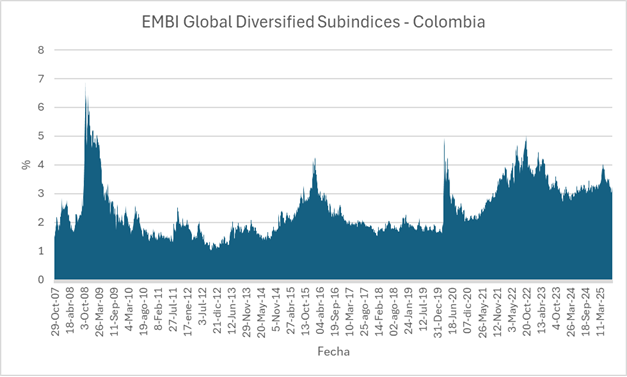
\includegraphics[width=0.9\textwidth]{graficas/embi.png}
  \end{center}
\end{frame}

\begin{frame}
  \frametitle{Riesgo País}
  \begin{center}
    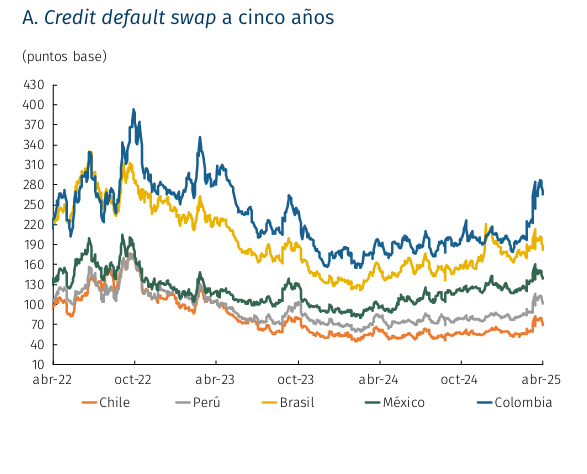
\includegraphics[width=0.7\textwidth]{graficas/cds.png}
    %\vspace{0.2cm}
    %\scriptsize\textit{Fuente: Informe de Política Monetaria Banco de la República.}
  \end{center}
\end{frame}


%\begin{frame}
%  \frametitle{Riesgo País}
%  \begin{center}
%    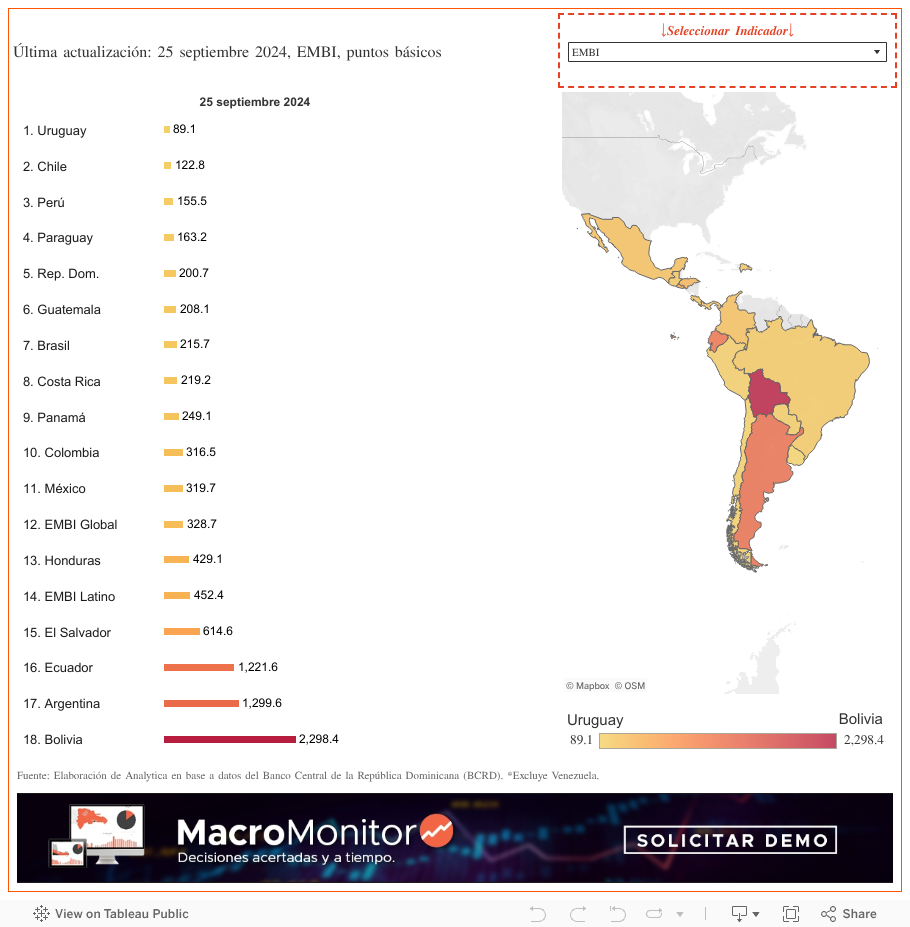
\includegraphics[width=0.7\textwidth]{graficas/1_rss.png}
%  \end{center}
%\end{frame}

%%\begin{frame}{Balance del GNC — Pronóstico PGN 2024 vs Cierre 2024}
\scriptsize
\begin{table}[h!]
\centering
\caption{Balance del GNC. Pronóstico PGN 2024 vs Cierre 2024 (\% PIB)}
\label{tab:PGN2024Cierre2024}
\begin{tabular}{|l|>{\centering\arraybackslash}p{2.8cm}|>{\centering\arraybackslash}p{2.8cm}|>{\centering\arraybackslash}p{2.8cm}|}
\hline
 & \textbf{Act PF PGN 2024 (Pronóstico)} & \textbf{Cierre 2024 (Resultado)} & \textbf{\textit{Diferencia}} \\
\hline
\textbf{Ingresos tributarios}   & 18,6 & 14,4 & \textit{-4,2} \\
\textbf{Otros ingresos}         & 2,1  & 2,1  & \textit{0,0} \\
\hline
\textbf{Gasto primario}         & 20,6 & 18,9 & \textit{-1,7} \\
\textbf{Intereses}              & 4,5  & 4,4  & \textit{-0,1} \\
\hline
\textbf{Déficit}                & 4,4  & 6,7  & \textit{2,3} \\
\hline
\end{tabular}
\vspace{0.3cm}
\par\footnotesize{\textit{Fuente: Actualización del Plan Financiero para el PGN 2024 y Balance Fiscal del GNC, Ministerio de Hacienda.}}
\end{table}
\end{frame}

%%\begin{frame}[fragile]
  \frametitle{Composición del Gasto por Nivel de Flexibilidad}

  \begin{table}[h!]
  \centering
  \scriptsize
  \begin{tabular}{@{}lcc@{}}
  \toprule
  \textbf{Categoría} & \textbf{2023} & \textbf{2024} \\
  \midrule
  \textbf{Gastos inflexibles}        & \textbf{20.1} & \textbf{20.7} \\
  \quad Intereses                    & 3.9  & 4.4  \\
  \quad Inversión                    & 1.4  & 1.3  \\
  \quad Gastos de personal           & 2.6  & 2.7  \\
  \quad SGP                          & 3.3  & 4.0  \\
  \quad Pensiones                    & 3.6  & 3.6  \\
  \quad Salud                        & 2.2  & 2.4  \\
  \quad FEPC                         & 1.7  & 1.2  \\
  \quad SENA, ICBF y otros           & 0.3  & 0.3  \\
  \quad Universidades                & 0.3  & 0.4  \\
  \quad Subsidios Serv. Públicos     & 0.3  & 0.2  \\
  \quad Cesantías y Salud FOMAG      & 0.1  & 0.1  \\
  \quad Deudas Entidades             & 0.3  & 0.1  \\
  \quad Sentencias                   & 0.1  & 0.1  \\
  \midrule
  \textbf{Gastos semiflexibles}      & \textbf{2.8}  & \textbf{2.5}  \\
  \quad Inversión                    & 1.2  & 0.7  \\
  \quad Adq. Bienes y Servicios      & 0.7  & 0.7  \\
  \quad Resto de transferencias      & 0.9  & 1.2  \\
  \quad FOME y FNG                   & 0.0  & 0.0  \\
  \bottomrule
  \end{tabular}
  \end{table}
%  \vspace{0.2cm}
%  \textit{Fuente: Cálculos propios con base en CARF y MHCP.}
\end{frame}

%%\begin{frame}{Balance del GNC — Cierre 2024 vs Plan Financiero 2025}
\scriptsize
\begin{table}[h!]
\centering
\caption{Balance del GNC. Cierre 2024 vs Act PF 2025 (\% PIB)}
\label{tab:Cierre2024PF2025}
%\resizebox{\textwidth}{!}{%
\begin{tabular}{|l|>{\centering\arraybackslash}p{3cm}|>{\centering\arraybackslash}p{3cm}|c|}
\hline
 & \textbf{Cierre 2024 (Resultado)} & \textbf{Act PF 2025 (Pronóstico)} & \textit{\textbf{Diferencia}} \\
\hline
\textbf{Ingresos tributarios}   & 14,4 & 15,5 &  \textit{1,1} \\
\textbf{Otros ingresos}         & 2,1  & 1,5  & \textit{-0,6} \\
\hline
\textbf{Gasto primario}         & 18,9 & 19,5 &  \textit{0,6} \\
\textbf{Intereses}              & 4,4  & 4,7  &  \textit{0,3} \\
\hline
\textbf{Déficit}                & 6,7  & 7,1  & \textit{0,4} \\
\hline
\end{tabular}%
%}
\vspace{0.3cm} 
\par\footnotesize{\textit{Fuente: Balance Fiscal del GNC y Act PF Jul 2025, Ministerio de Hacienda.}}
\end{table}
\end{frame}
%%\begin{frame}{Balance del GNC — Cierre 2024 vs Plan Financiero 2026}
\scriptsize
\begin{table}[h!]
\centering
\caption{Balance del GNC. Cierre 2024 vs Act PF 2026 (\% PIB)}
\label{tab:Cierre2024PF2025}
%\resizebox{\textwidth}{!}{%
\begin{tabular}{|l|>{\centering\arraybackslash}p{3cm}|>{\centering\arraybackslash}p{3cm}|c|}
\hline
 & \textbf{Cierre 2024 (Resultado)} & \textbf{Act PF 2026 (Pronóstico)} & \textit{\textbf{Diferencia}} \\
\hline
\textbf{Ingresos tributarios}   & 14,4 & 17,0 &  \textit{2,6} \\
\textbf{Otros ingresos}         & 2,1  & 1,6  & \textit{-0,5} \\
\hline
\textbf{Gasto primario}         & 18,9 & 20,6 &  \textit{1,7} \\
\textbf{Intereses}              & 4,4  & 4,2  &  \textit{-0,2} \\
\hline
\textbf{Déficit}                & 6,7  & 6,2  & \textit{-0,5} \\
\hline
\end{tabular}%
%}
\vspace{0.3cm} 
\par\footnotesize{\textit{Fuente: Balance Fiscal del GNC y Act PF Jul 2025, Ministerio de Hacienda.}}
\end{table}
\end{frame}

%\begin{frame}
\frametitle{Deuda neta del GNC}
\centering
\begin{tikzpicture}
\begin{axis}[
    width=12.6cm, height=5.7cm,
    clip=false,
    ylabel={\% del PIB},
    xmin=2019, xmax=2035.25,
    xtick={2019,2021,...,2035},
    xticklabel style={/pgf/number format/.cd,1000 sep={},fixed,precision=0},
    scaled x ticks=false,
    scaled y ticks=false,
    tick label style={font=\footnotesize},
    ylabel style={font=\small},
    ymajorgrids=true,
    grid style={dashed,black!20},
    unbounded coords=discard,
    filter discard warning=false,
    legend style={at={(0.5,1.035)},anchor=south,legend columns=4,
                  font=\scriptsize,draw=none,fill=none},
    legend cell align=left,
    ymin=40, ymax=115,
    ytick={40,50,...,110}
]

\addplot[black,thick,mark=*,mark size=1.5pt,restrict x to domain=2019:2025]
    table[col sep=comma,x=year,y=deuda_actualizacion]{datos/escenarios_4_1_4_2.csv};
\addlegendentry{Histórico}

% El MFMP 2024 proyecta desde 2024; punto de enlace de 2023.
\addplot[blue,thick,dashed,mark=none,restrict x to domain=2023:2035]
    table[col sep=comma,x=year,y=deuda_mfmp2024]{datos/escenarios_4_1_4_2.csv};
\addlegendentry{MFMP 2024}

\addplot[red,thick,dashed,mark=square*,mark size=1.5pt,restrict x to domain=2025:2035]
    table[col sep=comma,x=year,y=deuda_actualizacion]{datos/escenarios_4_1_4_2.csv};
\addlegendentry{Actualización}

% Hasta 2027, la consolidación coincide con la actualización.
\addplot[gray!80!black,thick,dotted,mark=triangle*,mark size=2pt,
         restrict x to domain=2027:2035]
    table[col sep=comma,x=year,y=deuda_consolidacion]{datos/escenarios_4_1_4_2.csv};
\addlegendentry{Consolidación}

\addplot[black!55,thin,dashed,forget plot] coordinates {(2022,55) (2035,55)};
\node[anchor=north west,font=\scriptsize,text=black!65] at (axis cs:2028,55) {Ancla: 55\%};
\addplot[black!55,thin,dotted,forget plot] coordinates {(2022,71) (2035,71)};
\node[anchor=south west,font=\scriptsize,text=black!65] at (axis cs:2022,71) {Límite: 71\%};

\node[anchor=west,font=\footnotesize,text=red] at (axis cs:2035.5,107.579448737) {107,6};
\node[anchor=west,font=\footnotesize,text=gray!80!black] at (axis cs:2035.5,65.5607778148) {65,6};
\node[anchor=south west,font=\footnotesize,text=blue] at (axis cs:2035.5,55.4) {55,4};
\end{axis}
\end{tikzpicture}

\par\vspace{0.05cm}
{\scriptsize Fuente: MHCP y cálculos propios.}\par
{\scriptsize Escenarios desde 2027: $r=5\%$ y $g=3\%$. La consolidación comienza en 2028.}
\note{[Sources] Figuras.xlsx, hoja 4.1, B2:R5; supuestos en J7:R9. MHCP: deuda neta del GNC y MFMP 2024; cálculos propios para actualización y consolidación. El MFMP 2024 proyecta desde 2024; las proyecciones actualizadas comienzan en 2026. Desde 2027, deuda/PIB = ((1+r)/(1+g)) por la deuda/PIB del año anterior menos el balance primario del año, con r=5\% y g=3\%. El balance primario proviene de la hoja 4.2. Actualización y consolidación coinciden hasta 2027. En 2035: MFMP 2024, 55,4\% del PIB; actualización, 107,5794\%; consolidación, 65,5608\%. Ancla: 55\%; límite: 71\%, referencias conservadas de la figura anterior.}
\end{frame}

%\begin{frame}
\frametitle{Balance primario del GNC}
\centering
\begin{tikzpicture}
\begin{axis}[
    width=12.6cm, height=5.7cm,
    clip=false,
    ylabel={\% del PIB},
    xmin=2019, xmax=2035.25,
    xtick={2019,2021,...,2035},
    xticklabel style={/pgf/number format/.cd,1000 sep={},fixed,precision=0},
    scaled x ticks=false,
    scaled y ticks=false,
    tick label style={font=\footnotesize},
    ylabel style={font=\small},
    ymajorgrids=true,
    grid style={dashed,black!20},
    unbounded coords=discard,
    filter discard warning=false,
    legend style={at={(0.5,1.035)},anchor=south,legend columns=2,
                  font=\scriptsize,draw=none,fill=none},
    legend cell align=left,
    ymin=-5.5, ymax=2,
    ytick={-5,-4,...,2}
]

\addplot[black,thick,mark=*,mark size=1.5pt,forget plot,
         restrict x to domain=2019:2025]
    table[col sep=comma,x=year,y=balance_actualizacion]{datos/escenarios_4_1_4_2.csv};

% Inercial corresponde al escenario Actualización de la hoja 4.2.
\addplot[red,thick,dashed,mark=square*,mark size=1.5pt,restrict x to domain=2025:2035]
    table[col sep=comma,x=year,y=balance_actualizacion]{datos/escenarios_4_1_4_2.csv};
\addlegendentry{Inercial}

% Hasta 2027, la consolidación coincide con el escenario inercial.
\addplot[gray!80!black,thick,dotted,mark=triangle*,mark size=2pt,
         restrict x to domain=2027:2035]
    table[col sep=comma,x=year,y=balance_consolidacion]{datos/escenarios_4_1_4_2.csv};
\addlegendentry{Consolidación}

\addplot[black!45,thin,forget plot] coordinates {(2019,0) (2035,0)};
\node[anchor=west,font=\footnotesize,text=gray!80!black] at (axis cs:2035.5,1.25423454585) {1,3};
\node[anchor=west,font=\footnotesize,text=red] at (axis cs:2035.5,-3.3) {-3,3};
\end{axis}
\end{tikzpicture}

\par\vspace{0.05cm}
{\scriptsize Fuente: MHCP y cálculos propios.}\par
{\scriptsize Datos hasta 2025 en línea continua. Ambos escenarios coinciden hasta 2027.}
\note{[Sources] Figuras.xlsx, hoja 4.2, B2:R2 (años 2019 a 2035), B4:R4 (Actualización) y B5:R5 (Consolidación). Inercial corresponde a Actualización en el Excel. MHCP: balance primario del GNC; cálculos propios para los escenarios inercial y de consolidación. Los datos hasta 2025 son comunes a los escenarios. Las proyecciones comienzan en 2026 y los escenarios coinciden hasta 2027. La consolidación comienza en 2028. En 2035: inercial, -3,3\% del PIB; consolidación, 1,2542\%. Desde 2028, el balance primario de consolidación es 0,2 + 0,1 por la diferencia entre la deuda del año anterior y 55, en puntos del PIB.}
\end{frame}

%%\begin{frame}
  \frametitle{Tenedores de Deuda Pública Interna - Dic 2019}

  \begin{figure}
    \centering
    \begin{tikzpicture}
      \pie[
        text=legend, 
        radius=2.5, % Adjusted size
        sum=100
      ]{
        31/{Fondos de Pensiones y Cesantías},
        24/{Fondos de Capital Extranjero},
        15/{Bancos Comerciales},
        15/{Entidades, Fiducias e Inst. Públicas},
        5/{Compañías de Seguros},
        10/{Otros}
      }
    \end{tikzpicture}
    \caption{Distribución de tenedores de deuda interna - Dic 2019}
    \label{fig:debt-holders-2019}
  \end{figure}

  \vspace{0.3cm}
  \footnotesize{\textit{Fuente: Cálculos con base en Dirección de Crédito Público del Ministerio de Hacienda.}}
\end{frame}

\begin{frame}
  \frametitle{Tenedores de Deuda Pública Interna - Dic 2024}

  \begin{figure}
    \centering
    \begin{tikzpicture}
      \pie[
        text=legend, 
        radius=2.5, % Adjusted size
        sum=100
      ]{
        32/{Fondos de Pensiones y Cesantías},
        18/{Fondos de Capital Extranjero},
        16/{Bancos Comerciales},
        12/{Entidades, Fiducias e Inst. Públicas},
        12/{Compañías de Seguros},
        10/{Otros}
      }
    \end{tikzpicture}
    \caption{Distribución de tenedores de deuda interna - Dic 2024}
    \label{fig:debt-holders-2024}
  \end{figure}

  \vspace{0.3cm}
  \footnotesize{\textit{Fuente: Cálculos con base en Dirección de Crédito Público del Ministerio de Hacienda.}}
\end{frame}

%\begin{frame}{Principales puntos del ajuste fiscal}
\begin{itemize}
    \item Deberá ser de más de \textbf{5 puntos del PIB}... pero probablemente más.
    \item Tiene que ser \textbf{gradual} para minimizar el impacto económico y social.
    \item Debe incluir políticas de \textbf{contención y reducción del gasto...}
    \item ... pero también incorporar políticas de  \textbf{aumento de los ingresos}.
%    \item La consolidación requiere posponer la Ley de Competencias que reglamenta el Acto Legislativo del SGP ....
%    \item ... o redefinir el SGP como \% del PIB.
    \item Se deben complementar con \textbf{reformas institucionales} y \textbf{políticas de crecimiento}.
\end{itemize}
\end{frame}


%\section{Riesgos}
%\begin{frame}
  \frametitle{Nómina de la Nación \small{(Anexos Presidenciales PGN)}}
  \begin{center}
    \begin{tabular}{lcccc}
        \hline
        \textbf{Sector} & \textbf{2023} & \textbf{2024} & \textbf{2025} & \textbf{2026} \\
        \hline
        \multicolumn{5}{c}{\textbf{Costo para la Nación (\% PIB)}} \\
        \hline
        Rama Ejecutiva (1) & 0.4 & 0.9 & 0.6 & 0.6 \\
        Militares y Policía (2) & 1.4 & 1.4 & 1.5 & 1.7 \\
        Leg / Jud / Fisc /  OrgAut (3) & 0.8 & 1.0 & 1.0 & 1.0 \\
        \textbf{Total PGN (1+2+3)} & \textbf{2.6} & \textbf{3.4} & \textbf{3.1} & \textbf{3.3} \\
        \hline
        SGP Educación (4) & 1.8 & 1.9 & 2.1 & 2.2 \\ 
        SGP Salud (5) & 0.2 & 0.2 & 0.2 & 0.2 \\
        Universidades (6) & 0.3 & 0.3 & 0.3 & 0.3 \\
        \textbf{Total Transferencias (4+5+6)}  & \textbf{2.3} & \textbf{2.4} & \textbf{2.6} & \textbf{2.7} \\
        \hline
        \textbf{Gran Total} & \textbf{4.9} & \textbf{5.8} & \textbf{5.8} & \textbf{6.0} \\
        \hline
    \end{tabular}
  \end{center}
\end{frame}

\begin{comment}
\begin{frame}
  \frametitle{Nómina de la Nación \small{(Anexos Presidenciales PGN)}}
  \begin{center}
    \begin{tabular}{lcccc}
        \hline
        \textbf{Sector} & \textbf{2023} & \textbf{2024} & \textbf{2025} & \textbf{2026} \\
        \hline
        \multicolumn{5}{c}{\textbf{Número de Cargos (miles)}} \\
        \hline
        Rama Ejecutiva (1) & 86 & 97 & 98 & 99 \\
        Defensa y Policía (2) & 498 & 496 & 511 & 480 \\
        Judicial, Fiscalía y Org. Aut. (3) & 80 & 84 & 88 & 88 \\
        \hline
        \textbf{Total PGN (1+2+3)} & \textbf{663} & \textbf{678} & \textbf{696} & \textbf{667} \\ \hline
        SGP Educación (4) & 353 & 356 & 362 & 362 \\ 
        SGP Salud (5) & 47 & 46 & 49 & 49 \\
        Universidades (6) & 59 & 59 & 55 & 55 \\ \hline
        \textbf{Total Transferencias (4+5+6)} & \textbf{459} & \textbf{461} & \textbf{467} & \textbf{475} \\ \hline
        \textbf{Gran Total} & \textbf{1122} & \textbf{1139} & \textbf{1163} & \textbf{1143} \\
        \hline
    \end{tabular}
  \end{center}
\end{frame}
\end{comment}

%\begin{frame}{Transferencias del GNC para pensiones y asignaciones de retiro}
\begin{center}
\begin{tikzpicture}
    \begin{axis}[
        width=10cm, height=6.5cm,
        xlabel={Año},
        ylabel={\% del PIB},
        xtick=data,
        ymin=0, ymax=3.5,
        legend pos=north west,
        grid=major,
        xticklabels={2024, 2025, 2026, 2027, 2028, 2029, 2030, 2031, 2032, 2033, 2034, 2035},
        xticklabel style={rotate=90, anchor=east},
        xlabel style={yshift=-15pt},
        ybar stacked,
        bar width=7pt,
        enlarge x limits={abs=0.5},
        nodes near coords style={font=\small}
    ]
    
    % Colpensiones
    \addplot[fill=white, draw=black] coordinates {
        (2024,1.40) (2025,1.54) (2026,1.61) 
        (2027,1.65) (2028,1.72) (2029,1.80) (2030,1.89) (2031,1.96) 
        (2032,1.99) (2033,2.04) (2034,2.07) (2035,2.11)
    };
    \addlegendentry{Colpensiones}
    
    % FF.AA.
    \addplot[fill=gray!70] coordinates {
        (2024,0.73) (2025,0.78) (2026,0.81) 
        (2027,0.82) (2028,0.84) (2029,0.86) (2030,0.90) (2031,0.91) 
        (2032,0.94) (2033,0.96) (2034,0.98) (2035,1.00)
    };
    \addlegendentry{FF. AA.}
    
    \end{axis}
\end{tikzpicture}
\end{center}
%\vspace{0.2cm}
%{\footnotesize\textit{Fuente: Marco Fiscal de Mediano Plazo 2024, Ministerio de Hacienda.}}
\end{frame}

%\begin{frame}{Transferencia del GNC a la ADRES*}
\begin{center}
\begin{tikzpicture}
    \begin{axis}[
        width=10cm, height=7cm,
 %       xlabel={Año},
        xlabel style={yshift=-15pt},
        ylabel={\% del PIB},
        xtick=data,
        grid=major,
        xticklabels={2024, 2025, 2026, 2027, 2028, 2029, 2030, 2031, 2032, 2033, 2034, 2035},
        xticklabel style={rotate=90, anchor=east},
        legend pos=north west,
        ymajorgrids=true,
        legend style={at={(0.03,0.97)}, anchor=north west}
    ]
    
    % Escenario Base
    \addplot[thick, color=blue, mark=*] coordinates {
        (2024,1.97) (2025,2.35) (2026,2.22) (2027,2.29) (2028,2.41) 
        (2029,2.51) (2030,2.62) (2031,2.73) (2032,2.85) (2033,2.97) 
        (2034,3.09) (2035,3.22)
    };
    \addlegendentry{Escenario Base}
    
    % Choque +1pp UPC
    \addplot[thick, color=red, mark=square*, style=dashed] coordinates {
        (2024,1.97) (2025,2.40) (2026,2.31) (2027,2.44) (2028,2.62) 
        (2029,2.77) (2030,2.95) (2031,3.12) (2032,3.31) (2033,3.50) 
        (2034,3.70) (2035,3.90)
    };
    \addlegendentry{Aumento anual 1pp UPC}
    
    \end{axis}
\end{tikzpicture}
\\{\footnotesize * No incluye los 4,4 puntos del antiguo CREE}%\\
\end{center}
%\vspace{0.1cm}
%{\footnotesize \textit{Fuente: Marco Fiscal de Mediano Plazo 2024, Ministerio de Hacienda.}}
\end{frame}

%\begin{frame}
  \frametitle{Transferencias del SGP como \% del PIB}

  \begin{figure}
    \centering
    \begin{tikzpicture}
        \begin{axis}[
            width=11cm, height=6.5cm,
            ylabel={\% del PIB},
            %xlabel={Año},
            xtick={2024,2025,2026,2027,2028,2029,2030,2031,2032,2033,2034,2035,2036,2037,2038},
            xticklabel style={rotate=90,anchor=east,/pgf/number format/.cd,1000 sep={},fixed,precision=0},
            scaled x ticks=false,
            ymin=3.5, ymax=6.5,
            ytick={4,4.5,5,5.5,6},
            grid=major,
            legend pos=north west,
        ]

        % MFMP 2024
        \addplot[color=blue, mark=*, dashed] coordinates {
            (2024,4.0) (2025,4.5) (2026,4.6) (2027,4.8)
            (2028,4.8) (2029,5.0) (2030,5.0) (2031,5.1) (2032,5.2)
            (2033,5.2) (2034,5.3) (2035,5.3)
        };
        \addlegendentry{MFMP 2024}

        % Acto Legislativo
        \addplot[color=red, mark=square*] coordinates {
            (2024,4.0) (2025,4.5) (2026,4.6) (2027,4.6)
            (2028,4.7) (2029,4.9) (2030,5.0) (2031,5.2) (2032,5.3)
            (2033,5.5) (2034,5.6) (2035,5.8) (2036,6.0) (2037,6.1) (2038,6.3)
        };
        \addlegendentry{Acto Legislativo}

        \end{axis}
    \end{tikzpicture}
  \end{figure}

\end{frame}

%\begin{frame}{Desafiós del SGP}
    \begin{itemize}
        \item La definición del SGP como \% de los ICN dificulta la consolidación fiscal.
        \item Reducir el déficit en 1.0 punto del PIB a través del aumento de los ICN requiere:
        \begin{itemize}
            \item $\frac{1}{1-0.25} = 1.333 \text{ puntos del PIB}$ si el SGP es el 25\% de los ICN
            \item $\frac{1}{1-0.395} = 1.652 \text{ puntos del PIB}$ si el SGP es el 39,5\% de los ICN
         
        \end{itemize}
    \end{itemize}
\end{frame}


%\begin{frame}{Riesgos Fiscales del Gasto}
\small
\begin{table}
\centering
\caption{Aumentos proyectados de los principales rubros 2025-2035}
\begin{tabular}{lcc}
\hline
\textbf{Rubro} & \textbf{Min} & \textbf{Max} \\
\hline
Gasto de personal & 0,0 & 0,7 \\
Pensiones         & 0,8 & 1,2 \\
Salud             & 1,2 & 1,9 \\
SGP               & 0,2 & 2,3 \\
\hline
\textbf{Total}    & \textbf{2,2} & \textbf{6,1} \\
\hline
\end{tabular}
\\ \vspace{0.4cm}
\footnotesize{\textit{Fuente: Elaboración propia con base en MFMP.}}
\end{table}
\end{frame}


%\section{Soluciones}
%\subsection{Medidas de Gastos}
%\begin{frame}{Medidas de gasto}
    \begin{itemize}
        \item \textbf{FEPC: } Eliminar subsidio al diésel.
        \item \textbf{Inversión:} 
        \begin{itemize}
            \item Mantener la suspensión de vigencias futuras.
            \item Llevar al mínimo el gasto de inversión discrecional.
            \item Flexibilizar APP.
        \end{itemize} 
        \item \textbf{Personal:} Revertir el aumento presupuestado del gasto de personal.
        \item \textbf{Salud:} 
        \begin{itemize}
            \item Acotar y condicionar los beneficios del PBS. 
            %\item El saneamiento de las finanzas del sector salud no puede darse a costa de las finanzas del GNC.
        \end{itemize} 
    \end{itemize}
\end{frame}

\begin{frame}{Medidas de gasto}
    \begin{itemize}
            \item \textbf{Pensiones:} 
            \begin{itemize}
                \item Reforma Paramétrica. 
                \item Impuesto a Pensiones, \item Contribuciones al Fondo de Solidaridad Pensional.
            \end{itemize}  
        \item \textbf{SGP:} 
        \begin{itemize}
            \item Aplazar la Ley de Competencias hasta que no culmine la consolidación fiscal.
            \item Preferiblemente introducir un nuevo Acto Legislativo para definir SGP como \% del PIB.
        \end{itemize}    
    \end{itemize}
\end{frame}

%\subsection{Medidas de Ingresos}
%\begin{frame}{Evolución del recaudo del IVA}
\centering
\begin{tikzpicture}
\begin{axis}[
    width=12cm,
    height=7cm,
%    xlabel={Año},
    ylabel={Recaudo de IVA (\% del PIB)},
    ymin=3.5, ymax=6,
    ytick={4,4.5,5,5.5,6},
    xtick={2012,2013,...,2024},
    xticklabel style={rotate=90, anchor=east, /pgf/number format/.cd,1000 sep={}}
]

% Serie de recaudo
\addplot+[mark=square*, solid] coordinates {
(2012,5.5)
(2013,4.9)
(2014,5.1)
(2015,5.2)
(2016,4.3)
(2017,4.9)
(2018,5.0)
(2019,5.2)
(2020,4.8)
(2021,5.2)
(2022,5.5)
(2023,5.3)
(2024,5.0)
};

% Línea punteada del promedio
\addplot[dashed, thick, gray] coordinates {(2012,5.1) (2024,5.1)};

\end{axis}
\end{tikzpicture}
\end{frame}

%\begin{frame}{Gasto Tributario como \% del PIB}
\begin{table}[H]
\centering
\begin{tabular}{lccc}
\toprule
\textbf{Año} & \textbf{2021} & \textbf{2022} & \textbf{2023} \\
\midrule
IVA              & 5.6 & 5.3 & 5.6 \\
Renta Naturales  & 1.5 & 1.6 & 1.6 \\
Renta Jurídicas  & 1.6 & 1.9 & 1.3 \\
\midrule
\textbf{Total}   & \textbf{8.7} & \textbf{8.8} & \textbf{8.5} \\
\bottomrule
\end{tabular}
\caption*{\footnotesize Fuente: Elaboración propia con base en Marcos Fiscales de Mediano Plazo.}
\end{table}
\end{frame}

\begin{comment}
\begin{frame}{Gasto Tributario como \% del PIB}
\begin{table}[H]
\centering
\begin{tabular}{lccccc}
\toprule
\textbf{Año} & \textbf{2020} & \textbf{2021} & \textbf{2022} & \textbf{2023} & \textbf{2023-2020} \\
\midrule
IVA              & 5.5 & 5.6 & 5.3 & 5.6 & 0.1 \\
Renta Naturales  & 0.7 & 1.5 & 1.6 & 1.6 & 0.9 \\
Renta Jurídicas  & 1.0 & 1.6 & 1.9 & 1.3 & 0.3 \\
\midrule
\textbf{Total}   & \textbf{7.2} & \textbf{8.7} & \textbf{8.8} & \textbf{8.5} & \textbf{1.3} \\
\bottomrule
\end{tabular}
\caption*{\footnotesize Fuente: Elaboración propia con base en Marcos Fiscales de Mediano Plazo.}
\end{table}
\end{frame}
\end{comment}

\begin{frame}{Desagregación del gasto tributario del IVA (2023)}
\begin{table}[htbp]
\centering
\begin{tabular}{|l|c|}
\hline
\textbf{Categoría} & \textbf{\% PIB} \\
\hline
Exclusiones & 4,1 \\
Exenciones & 1,3 \\
Tarifa reducida del 5\% & 0,5 \\
No deducibilidad IVA bienes de inversión & -0,6 \\
\hline
\textbf{Total} & \textbf{5,3} \\
\hline
\end{tabular}
\vspace{0.2cm}

\footnotesize{\textit{Fuente: MFMP 2024, Ministerio de Hacienda.}}
\end{table}
\end{frame}

%\begin{frame}[fragile]
  \frametitle{Composición de los Ingresos y Rentas Líquidas de las Personas Naturales}

  \begin{table}
  \centering
  \scriptsize
  \begin{tabular}{lcc}
  \hline
\textbf{Tipo de renta} & \textbf{Como $\%$ del total de los ingresos brutos} & \textbf{Como $\%$ del total de renta líquidas} \\
  \hline
  Rentas de trabajo         & 38\% & 61\% \\
  Rentas no laborales       & 42\% & 17\% \\
  Pensiones                 & 7\%  & 12\% \\
  Ganancias ocasionales     & 7\%  & 3\%  \\
  Rentas de capital         & 5\%  & 6\%  \\
  Dividendos                & 1\%  & 1\%  \\
  \hline
  \end{tabular}
  \end{table}

  \vspace{0.2cm}
  \scriptsize\textit{Elaboración propia con base en estadísticas de la DIAN del año gravable 2023}

\end{frame}

%\begin{frame}[fragile]
  \frametitle{Recaudo del Resto de Impuestos como \% del PIB (2025)}

  \begin{table}
  \centering
%  \scriptsize
  \begin{tabular}{l c}
  \hline
  \textbf{Impuesto} & \textbf{\% del PIB} \\
  \hline
  GMF (4x1000)                                  & 0,8 \\
  Aranceles                                     & 0,3 \\
  Impuestos a los combustibles y al carbono     & 0,1 \\
  Impoconsumo                                   & 0,2 \\
  Régimen SIMPLE                                & 0,1 \\
  Patrimonio                                    & 0,1 \\
  Resto                                         & 0,2 \\
  \hline
  \textbf{Total}                                & \textbf{1,9} \\
  \hline
  \end{tabular}
  \end{table}

  \vspace{0.2cm}
  {\centering\scriptsize
  Fuente: Balance fiscal del GNC, Ministerio de Hacienda y cálculos propios.\par
  Resto incluye impuestos saludables y a los plásticos, retención en la fuente de inmuebles, normalización y otros.\par
  El total se calcula con cifras sin redondear.\par}
  \note{[Sources] Figuras.xlsx, hoja BGNC, W6 (2025) y W9:W26, consultada el 18 de septiembre de 2026. Valores en porcentaje del PIB, no fracciones. GMF: W17 = 0,79658383652749; aranceles: W25 = 0,34183744201066585; combustibles y carbono: W13 + W14 = 0,09977857535951763; consumo: W15 = 0,2255939069817974; SIMPLE: W19 = 0,08888410261127896; patrimonio: W20 = 0,06741130553297259. Resto: W16 + W18 + W21 + W22 + W26 = 0,24429421159476283, que incluye CREE (cero en 2025), normalización, retención en la fuente de inmuebles, impuestos saludables y a los plásticos y otros impuestos. Total: suma de los siete rubros = W9 - W11 - W12 - W24 = 1,8643833806184853. Se excluyen renta e IVA interno y externo. Cifras mostradas con un decimal; la suma de las cifras redondeadas es 1,8, mientras que el total sin redondear se aproxima a 1,9.}

\end{frame}

%\begin{frame}{Medidas de ingreso}
    \begin{itemize}
        \item \textbf{Gasto tributario:}         \begin{itemize}
            \item 8\% del PIB
        \end{itemize} 
        \item \textbf{Evasión y elusión:}  
        \begin{itemize}
            \item Otro 8\% del PIB!
        \end{itemize}
            \item \textbf{Renta Naturales:} 
            \begin{itemize}
                \item Las rentas laborales están sobrecargadas de aportes y contribuciones... 
                \item ... mas no otros tipos de renta!
            \end{itemize}
    \end{itemize}
\end{frame}


\begin{frame}{Medidas de ingreso}
    \begin{itemize}
        \item \textbf{IVA}         \begin{itemize}
            \item Disminuir la tarifa general...
            \item ... siempre y cuando se reduzca el gasto tributario.
        \end{itemize}
        \item \textbf{Renta Jurídicas}         \begin{itemize}
            \item Disminuir la tarifa general, siempre y cuando:
                \begin{itemize}
                    \item Se corrijan asimetrías horizontales y verticales
                    \item Se eliminen rentas de destinación específica
                \end{itemize}
        \end{itemize}

    \end{itemize}
\end{frame}

\begin{frame}{Medidas de ingreso}
    \begin{itemize}
        \item \textbf{Otros impuestos:}         \begin{itemize}
            \item Eliminar SIMPLE
            \item Eliminar Impoconsumo
            \item Suspender Impuesto al Patrimonio
        \end{itemize} 
        \item \textbf{Reforma Tributaria Territorial}
        \item \textbf{Economía Política de las Reformas Tributarias}
    \end{itemize}
\end{frame}

%%\begin{frame}{Estrategias de Reforma Tributaria}
\begin{itemize}
%    \item \textbf{Meta}: aumentar recaudo permanente en al menos 2\% del PIB.
    \item \textbf{Beneficios Tributarios}:
    \begin{itemize}
        %\item Revisar y desmontar beneficios tributarios más costosos (1,3\% PIB).
        %\item Elevar tasa mínima efectiva al 20\% sobre base tributaria.
        \item Reformar Estatuto Tributario para explicitar beneficios y eliminarlos por defecto.
        \item Eventual eliminación de beneficios cuyo gasto tributario no esté cuantificado dentro del PGN.
    \end{itemize}
\end{itemize}
\end{frame}

\begin{frame}{Estrategias de Reforma Tributaria}
\begin{itemize}
    \item \textbf{Renta personas jurídicas}:
    \begin{itemize}
        \item Revisar y desmontar beneficios tributarios más costosos (Hasta 1,3\% PIB).
        \item Elevar tasa mínima efectiva al 20\% sobre base tributaria.
        \item Reducir tarifa general mediante eliminación de rentas de destinación específica y traslado de competencias.
        \item Combatir uso indebido de empresas para gastos personales (Hasta 1\% PIB).
    \end{itemize}
\end{itemize}
\end{frame}

\begin{frame}{Estrategias de Reforma Tributaria}
\begin{itemize}    
    \item \textbf{Renta personas naturales}:
    \begin{itemize}
        \item Evitar mayor carga sobre rentas laborales.
        \item Mayor control a rentas no laborales con deducciones inusuales.
        \item Eliminar exención a pensiones.
        \item Eliminar doble tributación de dividendos
    \end{itemize}
\end{itemize}
\end{frame}

\begin{frame}{Estrategias de Reforma Tributaria}
\begin{itemize}
    \item \textbf{IVA} ({Hasta \raisebox{0.2ex}{\texttildelow}}5\% PIB):
    \begin{itemize}
        \item Ampliar base: pasar exentos a excluidos y eliminar tarifa del 5\%.
        \item Considerar bajar tarifa general del 19\% al 16\% con base más amplia.
        \item Implementar Registro Único de Ingresos para compensaciones focalizadas.
    \end{itemize}
    \item \textbf{Otros impuestos}:
    \begin{itemize}
        \item Ampliar base del GMF a transacciones móviles (0,2\% PIB).
        \item Aumentar ImpoCarbono %y/o eliminar subsidio a combustibles (0,6\% PIB).
        \item Eliminar Impoconsumo y SIMPLE por baja eficiencia (-0,3\% PIB).
        \item Suspender Impuesto al Patrimonio.
    \end{itemize}
\end{itemize}
\end{frame}



\begin{frame}{Estrategias de Reforma Tributaria}
\begin{itemize}    
    \item \textbf{Control y equidad}:
    \begin{itemize}
        %\item Combatir uso indebido de empresas para gastos personales (1\% PIB).
        \item Modernizar tecnología aduanera para reducir contrabando (0,5\% PIB).
    \end{itemize}
    \item \textbf{Economía Política}:
    \begin{itemize}    
        \item Discusión con las cortes sobre ``derechos adquiridos'' de las personas jurídicas.
        \item Ley de Cabildeo.
        \item Acción colectiva de los gremios.
    \end{itemize}
    \item \textbf{Reforma Tributaria Territorial}
\end{itemize}
\end{frame}

%\subsection{Reformas Institucionales}
%\begin{frame}{Reformas Institucionales}
\begin{itemize}
    %\item Endeudamiento elevado, déficits persistentes y presión creciente por transferencias obligatorias.
    \item Activación de la cláusula de escape (2025) revela límites del actual marco fiscal.
    \item Problema estructural: obligación de incluir todas las obligaciones legales de gasto sin contar con ingresos suficientes.
    \item Práctica recurrente: sobreestimación de ingresos para cuadrar el presupuesto.
\end{itemize}
\end{frame}

\begin{frame}{Reformas Institucionales}
\begin{itemize}
    \item Oficina de Asistencia Técnica Presupuestal (OATP): fortalecer capacidad técnica del Congreso y complementar al CARF.
    \item Validación independiente y vinculante de proyecciones de ingresos (CARF) y obligaciones legales de gasto (OATP).
    \item Mecanismo automático: Si la regla fiscal impide presupuestar todas las obligaciones legales de gasto,  declarar emergencia económica para decretar impuestos.
    \item Modificar art. 348 C.P. para que, si el Congreso no aprueba el PGN, se reconduzca el presupuesto anterior.
\end{itemize}
\end{frame}

%\begin{frame}{Reformas Institucionales}
%\begin{itemize}
%    \item Unificar presupuestos de funcionamiento e inversión en MinHacienda.
%    \item Medir ejecución presupuestal excluyendo transferencias a fiducias/patrimonios autónomos.
%    \item Reformar “pérdidas de apropiación” para permitir traslado parcial de saldos no comprometidos.
%    \item Clasificación de Transacciones de Única Vez a cargo exclusivo del CARF.
%    \item Acceso público y auditable al detalle del cierre fiscal.
%\end{itemize}
%\end{frame}


%%\subsubsection{Inversión}
%%\begin{frame}{Inversión}
\begin{itemize}
    \item La reducción de la inversión por parte del GNC implicaría frenar proyectos de transporte, vivienda y territorio.
    \item Alternativas:
    \begin{itemize}
        \item Transferir competencias de inversión a las ET junto con recursos equivalentes vía SGP, con el GNC como coordinador y asistente técnico.
        \item Mayor concurrencia del sector privado.
        \item Relanzar las APP con incentivos ligados a calidad, topes a VF y pagos sujetos a ejecución.
        \item Ampliar el universo de APP reduciendo el umbral mínimo de inversión.
    \end{itemize}
\end{itemize}
\end{frame}

%%\subsubsection{FEPC}
%%\begin{frame}{Subsidio a los combustibles}
\begin{itemize}
    \item Transferencia al FEPC: 1,7\% del PIB (2023), 1,2\% (2024), 0,6\% (2025, proyectado).
    \item Eliminación implica suprimir subsidio al diésel: costo político, social y de orden público.
    \item MFMP 2024 prevé extinción total en 2026 → no representa nuevo aporte a la consolidación fiscal.
    \item Mantener objetivo de eliminación definitiva por razones fiscales y ambientales.
\end{itemize}
\end{frame}

%%\subsubsection{Pensiones}
%%\subsubsection{Salud}
%%\begin{frame}{Salud}
\begin{itemize}
    %\item Fortalecer programas de atención primaria y prevención para reducir enfermedades crónicas.
    \item Excluir tratamientos de bajo impacto o alto costo.
    \item Sistematizar y centralizar información de pacientes y tratamientos para mejorar gestión.
%\end{itemize}
%\end{frame}

%\begin{frame}{Salud}
%\begin{itemize}
%    \item Transición hacia competencia en primas entre EPS para incentivar eficiencia.
    \item Aumentar financiación territorial en el marco de la Ley de Competencias.
    \item Redirigir contribuciones a Cajas de Compensación al Sistema de Salud.
%\end{itemize}
%\end{frame}

%\begin{frame}{Salud}
%\begin{itemize}
    \item Aumentar cotización a salud de pensionados al 16\%.
 %   \item Financiar salud con impuestos generales (ej. IVA) eliminando exenciones y tarifas diferenciadas.
%    \item Reconocer que, aunque se contenga el gasto, la presión fiscal del sector salud seguirá en aumento por envejecimiento y nuevas tecnologías.
\end{itemize}
\end{frame}

%%\begin{frame}{Pensiones}
\begin{itemize}
%    \item El gasto pensional no se limita a Colpensiones: incluye regímenes especiales (FFAA, docentes, empleados públicos).
%    \item Las asignaciones de retiro de FFAA siguen vigentes y presionan las finanzas públicas.
%    \item 2024–2035: gasto en pensiones +1 pp PIB (Colpensiones +0,7 pp; asignaciones de retiro +0,3 pp).
    \item Baja cobertura: sólo 1 de cada 4 adultos mayores recibe pensión.
%\end{itemize}
%\end{frame}

%\begin{frame}{Pensiones}
%\begin{enumerate}
    \item Ajustes paramétricos: 
    \begin{itemize}
        \item Edad de pensión
        \item Tasa de reemplazo
        \item Umbral de cotización
    \end{itemize}    
    %\item Contener el aumento del salario mínimo.
    \item Eliminar la exención de impuestos a las pensiones.
    \item Aumentar cotización en salud de los pensionados.
    \item Incrementar aportes de los pensionados al Fondo de Solidaridad Pensional.
    %\item Eliminar pensiones múltiples financiadas con recursos públicos.
\end{itemize}
\end{frame}

%\begin{frame}{Pensiones}
%\begin{itemize}
%    \item Ley 2381 de 2024: más cotizaciones al componente público; fondo de ahorro en BanRep.
%    \item Riesgo de uso de los recursos del fondo ante presiones fiscales → agotamiento proyectado en 2064.
%    \item Necesarios ajustes paramétricos: umbral de ingresos, tasa de reemplazo, edad de jubilación por cohortes.
%    \item Implementar pronto → señal de compromiso fiscal; reducción de pasivo implícito y riesgo país.
%\end{itemize}
%\end{frame}

%%\subsubsection{SGP}
%%\begin{frame}{SGP}
\begin{table}[h!]
\centering
\caption{Costo de competencias del GNC transferibles a los ET (2024)}
\begin{tabular}{|l|c|}
\hline
\textbf{Competencia} & \textbf{\% del PIB} \\
\hline
Inversión & 2,0 \\
Salud* & 2,4 \\
SENA e ICBF** & 0,2 \\
Universidades & 0,4 \\
\hline
\textbf{Total} & \textbf{5,0} \\
\hline
\end{tabular}
\end{table}
\vspace{0.1cm}
\\{\footnotesize *Incluye 4,4 de los 9 puntos porcentuales del impuesto a la renta del antiguo CREE.}\\
{\footnotesize **Corresponde a 3,6 de los 9 puntos porcentuales del impuesto a la renta del antiguo CREE.}
\end{frame}

%%\begin{frame}{SGP}
\begin{itemize}
    \item Algunos riesgos del Acto Legislativo que aumenta el SGP son subsanables mediante la ley de competencias...
    \item ... pero otros no.
    \item Si $s$ es la participación del SGP en los ICN, entonces un ajuste fiscal de 1 punto del PIB por el lado de los ingresos debe recaudar $\frac{1}{1-s}$ puntos del PIB.
    \item El Acto Legislativo llega en el peor momento.
    \item  La consolidación requiere posponer la Ley de Competencias que reglamenta el Acto Legislativo del SGP ...
    \item ... o redefinir el SGP como \% del PIB, lo cual requeriría otro acto legislativo.
\end{itemize}
\end{frame}

%%\begin{comment}
% ===============================
% Slide 1: Impacto fiscal del SGP
% ===============================
\begin{frame}{Sistema General de Participaciones (SGP)}
\begin{itemize}
  \item El SGP atado a los ingresos corrientes de la Nación genera un \textbf{automatismo de gasto}: mayores ingresos ⇒ mayores transferencias.
  \item Con el Acto Legislativo, el SGP pasará de \textbf{4,0\% del PIB en 2024} a \textbf{6,3\% en 2038}.
  \item Una reforma tributaria orientada a consolidación fiscal pierde eficacia, pues parte del nuevo recaudo se destina al SGP.
\end{itemize}
\end{frame}

% ===============================
% Slide 2: Traslado de competencias
% ===============================
\begin{frame}{Ley de Competencias: Traslado de funciones}
\begin{itemize}
  \item Para contener el impacto fiscal del Acto Legislativo, se requiere que las ET asuman nuevas responsabilidades.
  \item Posibles competencias a transferir:
  \begin{itemize}
    \item Inversión pública (2,0\% del PIB).
    \item Salud (2,4\% del PIB).
    \item SENA e ICBF (0,2\% del PIB).
    \item Universidades públicas (0,4\% del PIB).
  \end{itemize}
  \item Transferencia fiscalmente viable solo si va acompañada de transferencia de competencias equivalentes.
\end{itemize}
\end{frame}
\end{comment}


% ===============================
% Slide 3: Sobretasas locales
% ===============================
\begin{frame}{Autonomía Tributaria Territorial}
\begin{itemize}
  \item Se propone dotar a las ET de la capacidad para establecer sobretasas sobre:
  \begin{itemize}
    \item El Impuesto al Valor Agregado (IVA).  
    \item El Impuesto a la Renta.  
  \end{itemize}
  \item Prerequisito: Fondo de Compensación.
%\end{itemize}

%\begin{itemize}
%  \item Avanzar en \textbf{autonomía tributaria territorial}.
  \item Propuesta en IVA:
  \begin{itemize}
    \item Reducir tarifa general del IVA (19\% → 16\%).
    \item Eliminar ICA
    \item Permitir a distritos y departamentos fijar una sobretasa local.
  \end{itemize}
%  \item Incentivos: los territorios se benefician directamente del recaudo adicional generado por formalización y control.
\end{itemize}
\end{frame}

% ===============================
% Slide 3: Sobretasas locales
% ===============================
\begin{frame}{Autonomía Tributaria Territorial}
\begin{itemize}
%  \item Avanzar en \textbf{autonomía tributaria territorial}.
  \item Propuesta en renta jurídicas:
  \begin{itemize}
    \item Reducir tarifa general de renta jurídica en hasta 9 puntos 
    \item Permitir que las entidades territoriales puedan poner una sobretasa de hasta 9 puntos 
    \item Eliminar rentas de destinación específica del antiguo CREE
    \item Reasignar competencias del antiguo CREE 
    \begin{itemize}
        \item 4,4 Salud
        \item 1,4 SENA
        \item 2,2 ICBF 
        \item 0,4 Infancia
        \item 0,6 Universidades
    \end{itemize}
    %\item Reducir tarifa general del IVA (19\% → 16\%).
    %\item Permitir a distritos y departamentos fijar \textbf{sobretasas locales}.
  \end{itemize}
%  \item Incentivos: los territorios se benefician directamente del recaudo adicional generado por formalización y control.
\end{itemize}
\end{frame}


\begin{comment}
% ===============================
% Slide 4: Fórmula del SGP
% ===============================
\begin{frame}{Revisar la fórmula del SGP}
\begin{itemize}
  \item Problema: definición del SGP como porcentaje de los ingresos corrientes de la Nación.
  \item Alternativas:
  \begin{enumerate}
    \item Redefinirlo como porcentaje del PIB (requiere reforma constitucional).
    \item Excluir ingresos adicionales de reformas tributarias, clasificándolos como \textbf{rentas de destinación específica} para el servicio de la deuda.
  \end{enumerate}
  \item Objetivo: evitar que las reformas tributarias pierdan eficacia y que se repita la “reforma cada dos años”.
\end{itemize}
\end{frame}
\end{comment}
%%\subsubsection{Resumen}

%\section{Comentarios Finales}
%\begin{comment}
\begin{frame}{Epílogo: Un desafío estructural}
\begin{itemize}
    \item La crisis fiscal actual es estructural: incapacidad de aumentar recaudo y retornar a la senda de gasto pre-pandemia.
    \item Requiere solución de Estado: superar barreras políticas, legales y constitucionales.
    \item Urgencia: evitar que la deuda pública alcance niveles inmanejables y que se intensifiquen presiones de gasto (intereses, SGP, pensiones, salud, personal).
    \item Retrasar el ajuste aumenta el costo social, económico y político.
\end{itemize}
\end{frame}

\begin{frame}{Ruta para la consolidación fiscal}
\begin{itemize}
    \item Ajuste superior a 4\% del PIB: reformas tributarias sucesivas, racionalización del gasto en salud, personal y pensiones.
    \item Compatibilidad de la Ley de Competencias del SGP con sostenibilidad fiscal.
    \item Evitar que nuevos ingresos tributarios se transfieran automáticamente vía SGP.
    \item Revisión profunda de beneficios tributarios, especialmente en IVA, con mecanismos de compensación a hogares vulnerables.
\end{itemize}
\end{frame}
\end{comment}

\begin{frame}{Comentarios Finales}
\begin{itemize}
%    \item Reformas institucionales.
    %\item Crecimiento económico sostenido como condición para estabilidad fiscal.
    \item Agenda pro-crecimiento: 
    \begin{itemize}
        \item Libre competencia
        \item Flexibilización laboral
        \item Modernización financiera 
        \item Asignación del riesgo
        \item Incentivos a la innovación
    \end{itemize}
    \item ¿Disyuntiva entre estabilidad financiera y control de la inflación?
    \item ¿Cómo vender la idea de pagar más impuestos y reducir el gasto?
\end{itemize}
\end{frame}

%\begin{frame}
  \frametitle{Tenedores de Deuda Pública Interna - Dic 2019}

  \begin{figure}
    \centering
    \begin{tikzpicture}
      \pie[
        text=legend, 
        radius=2.5, % Adjusted size
        sum=100
      ]{
        31/{Fondos de Pensiones y Cesantías},
        24/{Fondos de Capital Extranjero},
        15/{Bancos Comerciales},
        15/{Entidades, Fiducias e Inst. Públicas},
        5/{Compañías de Seguros},
        10/{Otros}
      }
    \end{tikzpicture}
    \caption{Distribución de tenedores de deuda interna - Dic 2019}
    \label{fig:debt-holders-2019}
  \end{figure}

  \vspace{0.3cm}
  \footnotesize{\textit{Fuente: Cálculos con base en Dirección de Crédito Público del Ministerio de Hacienda.}}
\end{frame}

\begin{frame}
  \frametitle{Tenedores de Deuda Pública Interna - Dic 2024}

  \begin{figure}
    \centering
    \begin{tikzpicture}
      \pie[
        text=legend, 
        radius=2.5, % Adjusted size
        sum=100
      ]{
        32/{Fondos de Pensiones y Cesantías},
        18/{Fondos de Capital Extranjero},
        16/{Bancos Comerciales},
        12/{Entidades, Fiducias e Inst. Públicas},
        12/{Compañías de Seguros},
        10/{Otros}
      }
    \end{tikzpicture}
    \caption{Distribución de tenedores de deuda interna - Dic 2024}
    \label{fig:debt-holders-2024}
  \end{figure}

  \vspace{0.3cm}
  \footnotesize{\textit{Fuente: Cálculos con base en Dirección de Crédito Público del Ministerio de Hacienda.}}
\end{frame}

%\begin{comment}
\begin{frame}{Epílogo: Un desafío estructural}
\begin{itemize}
    \item La crisis fiscal actual es estructural: incapacidad de aumentar recaudo y retornar a la senda de gasto pre-pandemia.
    \item Requiere solución de Estado: superar barreras políticas, legales y constitucionales.
    \item Urgencia: evitar que la deuda pública alcance niveles inmanejables y que se intensifiquen presiones de gasto (intereses, SGP, pensiones, salud, personal).
    \item Retrasar el ajuste aumenta el costo social, económico y político.
\end{itemize}
\end{frame}

\begin{frame}{Ruta para la consolidación fiscal}
\begin{itemize}
    \item Ajuste superior a 4\% del PIB: reformas tributarias sucesivas, racionalización del gasto en salud, personal y pensiones.
    \item Compatibilidad de la Ley de Competencias del SGP con sostenibilidad fiscal.
    \item Evitar que nuevos ingresos tributarios se transfieran automáticamente vía SGP.
    \item Revisión profunda de beneficios tributarios, especialmente en IVA, con mecanismos de compensación a hogares vulnerables.
\end{itemize}
\end{frame}
\end{comment}

\begin{frame}{Comentarios Finales}
\begin{itemize}
%    \item Reformas institucionales.
    %\item Crecimiento económico sostenido como condición para estabilidad fiscal.
    \item Agenda pro-crecimiento: 
    \begin{itemize}
        \item Libre competencia
        \item Flexibilización laboral
        \item Modernización financiera 
        \item Asignación del riesgo
        \item Incentivos a la innovación
    \end{itemize}
    \item ¿Disyuntiva entre estabilidad financiera y control de la inflación?
    \item ¿Cómo vender la idea de pagar más impuestos y reducir el gasto?
\end{itemize}
\end{frame}


\begin{frame}{}
\centering
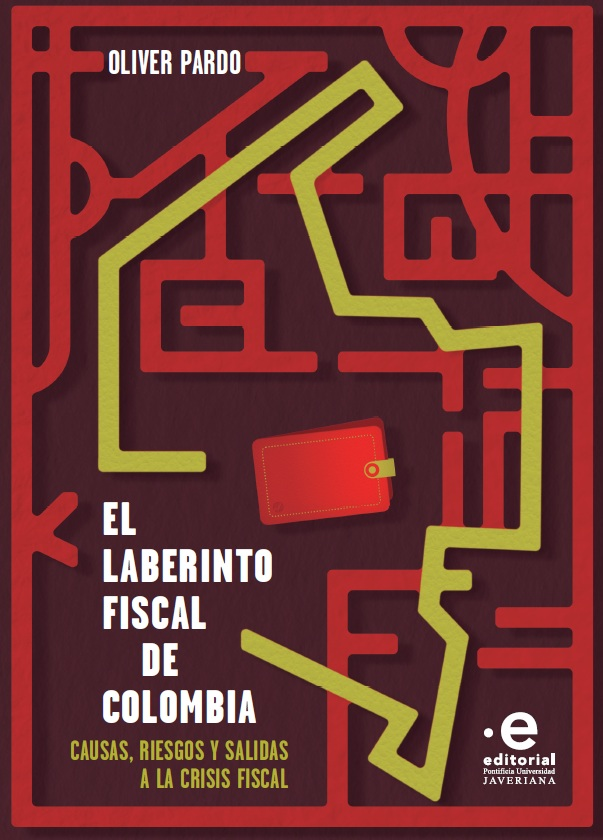
\includegraphics[scale=0.5]{graficas/Cover.jpg}
%
\includegraphics[scale=0.5]{graficas/QR.jpeg}
\end{frame}


%%\subsection{Medidas de Ingresos}
%%
\begin{frame}[fragile]
  \frametitle{Evolución del Recaudo de los Principales Impuestos (\% del PIB)}

%  \scriptsize
  \begin{table}
  \centering
  \begin{tabular}{|l|c|c|c|c|}
  \hline
  \textbf{Año} & \textbf{Renta*} & \textbf{IVA} & \textbf{Resto} & \textbf{Total} \\
  \hline
  2012 & 6,6 & 5,5 & 2,3 & \textbf{14,3} \\
  2013 & 6,7 & 4,9 & 2,6 & \textbf{14,1} \\
  2014 & 6,6 & 5,1 & 2,5 & \textbf{14,2} \\
  2015 & 6,6 & 5,2 & 2,7 & \textbf{14,5} \\
  2016 & 6,8 & 4,3 & 2,4 & \textbf{13,6} \\
  2017 & 6,8 & 4,9 & 2,0 & \textbf{13,8} \\
  2018 & 7,1 & 5,0 & 1,5 & \textbf{13,7} \\
  2019 & 7,0 & 5,2 & 1,8 & \textbf{14,0} \\
  2020 & 6,8 & 4,8 & 1,5 & \textbf{13,1} \\
  2021 & 6,8 & 5,2 & 1,6 & \textbf{13,6} \\
  2022 & 7,2 & 5,5 & 1,7 & \textbf{14,4} \\
  2023 & 9,6 & 5,3 & 1,8 & \textbf{16,7} \\
  2024 & 7,5 & 5,0 & 1,9 & \textbf{14,4} \\
  \hline
  \end{tabular}
%  \vspace{0.1cm}

  \par\footnotesize{* Incluye recaudo del CREE entre 2013 y 2016.}
%  \par\footnotesize{\textit{Fuente: Balance General del GNC, Ministerio de Hacienda.}}
  \end{table}

\end{frame}


%%\begin{frame}{Recaudo esperado de reformas tributarias}
\begin{table}[h]
    \caption{Recaudo esperado de reformas tributarias}
    \label{tab:tax:summ}
    \centering
    \begin{tabular}{|c|c|}
        \hline
        \textbf{Ley} & \textbf{Recaudo Esperado (\% PIB)} \\
        \hline
        Ley 1943 de 2018 & 1.2 \\
        \hline
        Ley 2155 de 2021 & 1.5 \\
        \hline
        Ley 2277 de 2022 & 2.0 \\
        \hline
        %\textbf{Total} & \textbf{4.7} \\
        %\hline
    \end{tabular}
\vspace{0.3cm}
\par\footnotesize{\textit{Fuente: Cálculos con base en exposiciones de motivos.}}    
\end{table}
\end{frame}

%%\begin{frame}{Desagregación del gasto tributario del IVA (2023)}
\begin{table}[h]
\centering
\begin{tabular}{|l|c|}
\hline
\textbf{Categoría} & \textbf{\% PIB} \\
\hline
Exclusiones & 4,1 \\
Exenciones & 1,3 \\
Tarifa reducida del 5\% & 0,5 \\
No deducibilidad IVA bienes de inversión & -0,6 \\
\hline
\textbf{Total} & \textbf{5,3} \\
\hline
\end{tabular}
\vspace{0.1cm}
\par \footnotesize{\textit{Fuente: MFMP 2024, Ministerio de Hacienda.}}
\end{table}
\end{frame}




%%\begin{frame}{Nómina de la Nación presupuestada para 2025}
\scriptsize
\begin{table}[h!]
\centering
\caption{Nómina de la Nación presupuestada para 2025}
\label{tab:Personal}
\begin{tabular}{|>{\arraybackslash}p{7cm}|>{\centering\arraybackslash}p{2cm}|>{\centering\arraybackslash}p{2cm}|}
\hline
\textbf{Sector} & \textbf{Cargos (Miles)} & \textbf{Costo (\% PIB)} \\ \hline
1. Rama Ejecutiva & 98 & 0,6 \\ 
2. Militares y Policía & 511 & 1,5 \\ 
3. Judicial, Legislativa y otros & 88 & 1,0 \\ \hline
\textbf{Financiación x PGN (1+2+3)} & \textbf{696} & \textbf{3,1} \\ \hline
4. SGP Educación & 362 & 2,1 \\ 
5. SGP Salud & 49 & 0,2 \\ 
6. Universidades & 55 & 0,3 \\ \hline
\textbf{Financiación x Transferencias (4+5+6)} & \textbf{467} & \textbf{2,6} \\ \hline
\textbf{Gran Total} & \textbf{1163} & \textbf{5,8} \\ \hline
\end{tabular}
\vspace{0.3cm}
\par\footnotesize{\textit{Fuente: Elaboración propia con base en el Anexo Presidencial del PGN 2025.}}
\end{table}
\end{frame}

%%\begin{frame}
\frametitle{Vigencias futuras e inversión pública (\% PIB)}

\begin{figure}
    \centering
    \begin{tikzpicture}
        \begin{axis}[
            width=0.85\textwidth,
            height=0.55\textwidth,
            grid=major,
 %           xlabel={Año},
            ylabel={\% PIB},
            ymin=0.5, ymax=3.0,
            xtick={2019,2020,2021,2022,2023,2024,2025},
            xticklabel style={rotate=90,anchor=east,/pgf/number format/.cd,1000 sep={},fixed,precision=0},
            scaled x ticks=false,
            ytick={0.50,0.75,1.00,1.25,1.50,1.75,2.00,2.25,2.50,2.75},
            legend pos=north west,
            ymajorgrids=true,
            xmajorgrids=true,
            grid style=dashed,
        ]

        % Vigencias futuras
        \addplot[
            color=blue,
            mark=square,
            thick
        ]
        coordinates {
            (2019,0.8)
            (2020,0.8)
            (2021,0.9)
            (2022,1.1)
            (2023,0.9)
            (2024,1.0)
            (2025,1.2)
        };

        % Inversión pública
        \addplot[
            color=red,
            mark=triangle,
            dashed,
            thick
        ]
        coordinates {
            (2019,1.7)
            (2020,2.0)
            (2021,2.2)
            (2022,2.7)
            (2023,2.6)
            (2024,2.0)
        };

        \legend{Vigencias futuras, Inversión pública}

        \end{axis}
    \end{tikzpicture}

    \vspace{0.3cm}
%    \par\footnotesize{\textit{Fuente: Elaboración propia con base en Marcos Fiscales de Mediano Plazo 2018--2024 y Balance del GNC, Ministerio de Hacienda.}}
\end{figure}

\end{frame}

%%
\begin{frame}
  \frametitle{Riesgo País}
  \begin{center}
    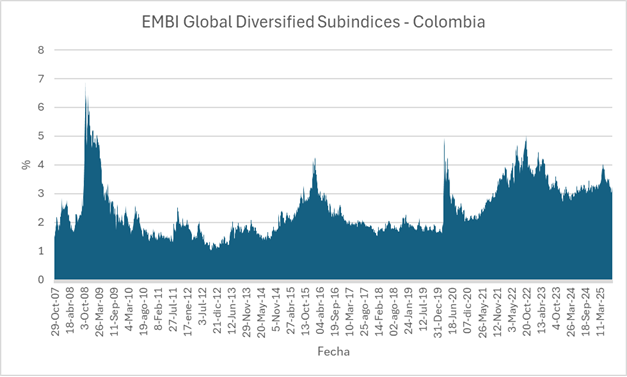
\includegraphics[width=0.9\textwidth]{graficas/embi.png}
  \end{center}
\end{frame}

\begin{frame}
  \frametitle{Riesgo País}
  \begin{center}
    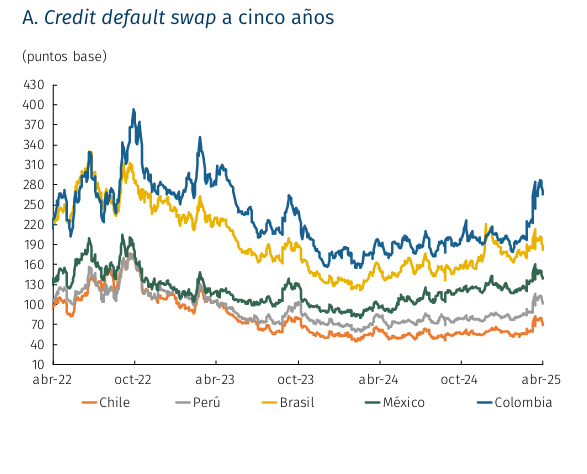
\includegraphics[width=0.7\textwidth]{graficas/cds.png}
    %\vspace{0.2cm}
    %\scriptsize\textit{Fuente: Informe de Política Monetaria Banco de la República.}
  \end{center}
\end{frame}


%\begin{frame}
%  \frametitle{Riesgo País}
%  \begin{center}
%    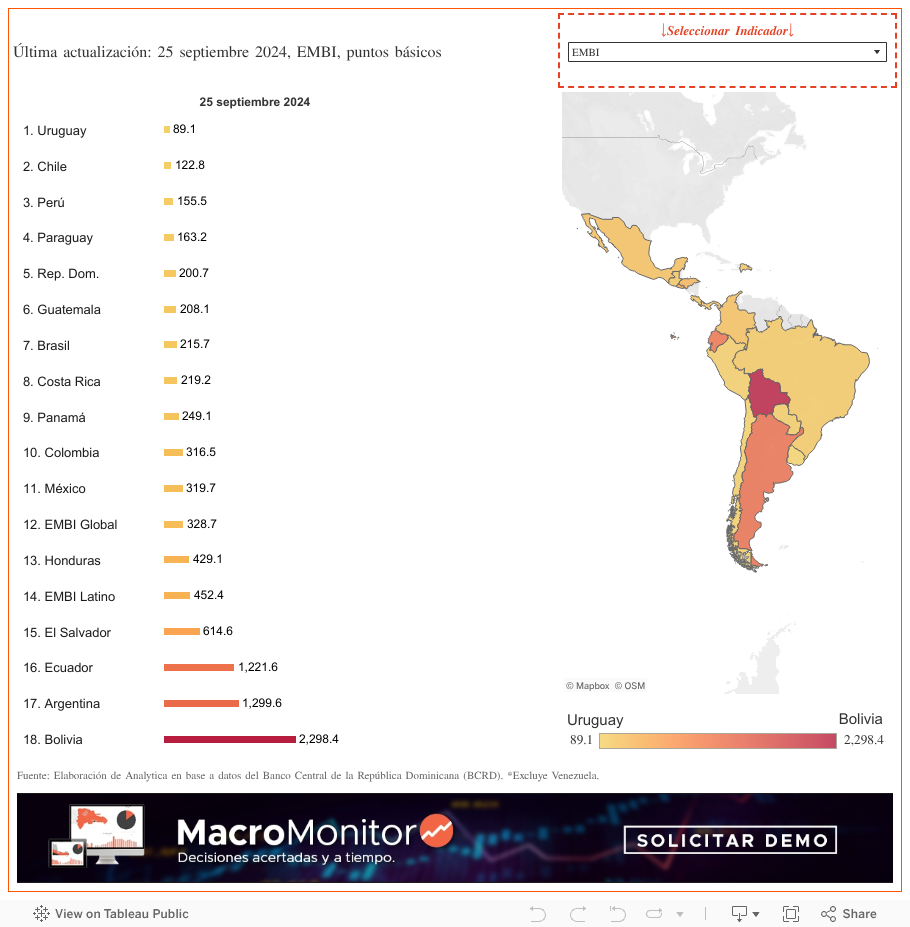
\includegraphics[width=0.7\textwidth]{graficas/1_rss.png}
%  \end{center}
%\end{frame}

%\begin{frame}{Balance del GNC — Pronóstico PGN 2024 vs Cierre 2024}
\scriptsize
\begin{table}[h!]
\centering
\caption{Balance del GNC. Pronóstico PGN 2024 vs Cierre 2024 (\% PIB)}
\label{tab:PGN2024Cierre2024}
\begin{tabular}{|l|>{\centering\arraybackslash}p{2.8cm}|>{\centering\arraybackslash}p{2.8cm}|>{\centering\arraybackslash}p{2.8cm}|}
\hline
 & \textbf{Act PF PGN 2024 (Pronóstico)} & \textbf{Cierre 2024 (Resultado)} & \textbf{\textit{Diferencia}} \\
\hline
\textbf{Ingresos tributarios}   & 18,6 & 14,4 & \textit{-4,2} \\
\textbf{Otros ingresos}         & 2,1  & 2,1  & \textit{0,0} \\
\hline
\textbf{Gasto primario}         & 20,6 & 18,9 & \textit{-1,7} \\
\textbf{Intereses}              & 4,5  & 4,4  & \textit{-0,1} \\
\hline
\textbf{Déficit}                & 4,4  & 6,7  & \textit{2,3} \\
\hline
\end{tabular}
\vspace{0.3cm}
\par\footnotesize{\textit{Fuente: Actualización del Plan Financiero para el PGN 2024 y Balance Fiscal del GNC, Ministerio de Hacienda.}}
\end{table}
\end{frame}

%\begin{frame}{Depósitos del Tesoro Nacional \small{(Fuente: Cálculos propios con base en MHCP)}} 
\begin{figure}
\centering
%\caption{Depósitos del Tesoro Nacional}
\label{fig:depositos}
\begin{tikzpicture}
\begin{axis}[
    width=0.8\textwidth,
    height=0.5\textwidth,
    ylabel={ \$ Billones de sep. 2025},
    xtick={1,2,3,4,5,6,7,8,9,10,11,12},
    xticklabels={Ene,Feb,Mar,Abr,May,Jun,Jul,Ago,Sep,Oct,Nov,Dic},
    xticklabel style={rotate=90, anchor=east},
    legend columns=3,
    legend style={at={(0.5,1.05)},anchor=south},
    clip=false,
    grid=both,
    legend style={font=\footnotesize},
    ymin=0
]

% Valores de 2025
\addplot coordinates {
    (1,19) (2,11) (3,10) (4,14) (5,16) (6,6) 
    (7,8) (8,7) (9,17) 
};
\addlegendentry{2025}


% Valores de 2024
\addplot coordinates {
    (1,21) (2,11) (3,14) (4,8) (5,18) (6,12) 
    (7,16) (8,16) (9,28) (10,20) (11,14) (12,4)
};
\addlegendentry{2024}

% Prom 2017 a 2023
\addplot[mark=square*, color=black, solid] coordinates {
    (1,34) (2,31) (3,30) (4,35) (5,44) (6,40)
    (7,40) (8,39) (9,43) (10,40) (11,35) (12,15)
};
\addlegendentry{Prom. 2017--2023}

\end{axis}
\end{tikzpicture}
\vspace{0.1cm}
%\par\footnotesize{\textit{Fuente: Elaboración propia con base en datos de la Dirección de Crédito Público, Ministerio de Hacienda.}}
\end{figure}
\end{frame}

%\begin{frame}{Evolución de reservas \small{(compromisos del año anterior pendientes por obligar)}}
\begin{figure}[h!]
\centering
%\caption{Evolución de reservas (compromisos del año anterior pendientes por obligar)}
\label{fig:reservas}
\begin{tikzpicture}
    \begin{axis}[
        ybar,
        symbolic x coords={2019, 2020, 2021, 2022, 2023, 2024},
        xtick=data,
        xticklabel style={rotate=90, anchor=east},
        ylabel={\% PIB},
        ymin=0, ymax=3.5,
        bar width=15pt,
        nodes near coords,
        enlarge x limits=0.2
    ]
        \addplot coordinates {
            (2019,1.4)
            (2020,1.7)
            (2021,1.5)
            (2022,1.6)
            (2023,2.1)
            (2024,3.0)
        };
    \end{axis}
\end{tikzpicture}
\vspace{0.1cm}
%\par\footnotesize{\textit{Fuente: Elaboración propia con base en ejecución presupuestal del rezago con recursos de la Nación excluyendo deuda a enero de cada año, Ministerio de Hacienda.}}
\end{figure}
\end{frame}

%\begin{frame}[fragile]
  \frametitle{Composición del Gasto por Nivel de Flexibilidad}

  \begin{table}[h!]
  \centering
  \scriptsize
  \begin{tabular}{@{}lcc@{}}
  \toprule
  \textbf{Categoría} & \textbf{2023} & \textbf{2024} \\
  \midrule
  \textbf{Gastos inflexibles}        & \textbf{20.1} & \textbf{20.7} \\
  \quad Intereses                    & 3.9  & 4.4  \\
  \quad Inversión                    & 1.4  & 1.3  \\
  \quad Gastos de personal           & 2.6  & 2.7  \\
  \quad SGP                          & 3.3  & 4.0  \\
  \quad Pensiones                    & 3.6  & 3.6  \\
  \quad Salud                        & 2.2  & 2.4  \\
  \quad FEPC                         & 1.7  & 1.2  \\
  \quad SENA, ICBF y otros           & 0.3  & 0.3  \\
  \quad Universidades                & 0.3  & 0.4  \\
  \quad Subsidios Serv. Públicos     & 0.3  & 0.2  \\
  \quad Cesantías y Salud FOMAG      & 0.1  & 0.1  \\
  \quad Deudas Entidades             & 0.3  & 0.1  \\
  \quad Sentencias                   & 0.1  & 0.1  \\
  \midrule
  \textbf{Gastos semiflexibles}      & \textbf{2.8}  & \textbf{2.5}  \\
  \quad Inversión                    & 1.2  & 0.7  \\
  \quad Adq. Bienes y Servicios      & 0.7  & 0.7  \\
  \quad Resto de transferencias      & 0.9  & 1.2  \\
  \quad FOME y FNG                   & 0.0  & 0.0  \\
  \bottomrule
  \end{tabular}
  \end{table}
%  \vspace{0.2cm}
%  \textit{Fuente: Cálculos propios con base en CARF y MHCP.}
\end{frame}

%%\begin{frame}{Evolución de reservas \small{(compromisos del año anterior pendientes por obligar)}}
\begin{figure}[h!]
\centering
%\caption{Evolución de reservas (compromisos del año anterior pendientes por obligar)}
\label{fig:reservas}
\begin{tikzpicture}
    \begin{axis}[
        ybar,
        symbolic x coords={2019, 2020, 2021, 2022, 2023, 2024},
        xtick=data,
        xticklabel style={rotate=90, anchor=east},
        ylabel={\% PIB},
        ymin=0, ymax=3.5,
        bar width=15pt,
        nodes near coords,
        enlarge x limits=0.2
    ]
        \addplot coordinates {
            (2019,1.4)
            (2020,1.7)
            (2021,1.5)
            (2022,1.6)
            (2023,2.1)
            (2024,3.0)
        };
    \end{axis}
\end{tikzpicture}
\vspace{0.1cm}
%\par\footnotesize{\textit{Fuente: Elaboración propia con base en ejecución presupuestal del rezago con recursos de la Nación excluyendo deuda a enero de cada año, Ministerio de Hacienda.}}
\end{figure}
\end{frame}

%%\begin{frame}{Depósitos del Tesoro Nacional}
\begin{figure}
\centering
\caption{Depósitos del Tesoro Nacional}
\label{fig:depositos}
\begin{tikzpicture}
\begin{axis}[
    width=0.7\textwidth,
    height=0.4\textwidth,
    ylabel={Billones de pesos de 2019},
    xtick={1,2,3,4,5,6,7,8,9,10,11,12},
    xticklabels={Ene,Feb,Mar,Abr,May,Jun,Jul,Ago,Sep,Oct,Nov,Dic},
    xticklabel style={rotate=90, anchor=east},
    legend pos=north west,
    grid=both,
    legend style={font=\footnotesize},
    ymin=0
]

% Valores de 2024
\addplot coordinates {
    (1,14.5) (2,7.9) (3,9.9) (4,5.3) (5,12.2) (6,8.4) 
    (7,11.1) (8,11.2) (9,19.3) (10,13.8) (11,9.8) (12,2.7)
};
\addlegendentry{2024}

% Mínimos de 2019 a 2023
\addplot[mark=square*, color=red, dashed] coordinates {
    (1,21.5) (2,9.4) (3,11.8) (4,17.9) (5,22.4) (6,17.6) 
    (7,18.4) (8,17.1) (9,23.9) (10,24.8) (11,22.1) (12,5.1)
};
\addlegendentry{Mínimo 2019--2023}

\end{axis}
\end{tikzpicture}
\vspace{0.1cm}
%\par\footnotesize{\textit{Fuente: Elaboración propia con base en datos de la Dirección de Crédito Público, Ministerio de Hacienda.}}
\end{figure}
\end{frame}

%\begin{frame}{Balance del GNC — Cierre 2024 vs Plan Financiero 2025}
\scriptsize
\begin{table}[h!]
\centering
\caption{Balance del GNC. Cierre 2024 vs Act PF 2025 (\% PIB)}
\label{tab:Cierre2024PF2025}
%\resizebox{\textwidth}{!}{%
\begin{tabular}{|l|>{\centering\arraybackslash}p{3cm}|>{\centering\arraybackslash}p{3cm}|c|}
\hline
 & \textbf{Cierre 2024 (Resultado)} & \textbf{Act PF 2025 (Pronóstico)} & \textit{\textbf{Diferencia}} \\
\hline
\textbf{Ingresos tributarios}   & 14,4 & 15,5 &  \textit{1,1} \\
\textbf{Otros ingresos}         & 2,1  & 1,5  & \textit{-0,6} \\
\hline
\textbf{Gasto primario}         & 18,9 & 19,5 &  \textit{0,6} \\
\textbf{Intereses}              & 4,4  & 4,7  &  \textit{0,3} \\
\hline
\textbf{Déficit}                & 6,7  & 7,1  & \textit{0,4} \\
\hline
\end{tabular}%
%}
\vspace{0.3cm} 
\par\footnotesize{\textit{Fuente: Balance Fiscal del GNC y Act PF Jul 2025, Ministerio de Hacienda.}}
\end{table}
\end{frame}
%\begin{frame}{Balance del GNC — Cierre 2024 vs Plan Financiero 2026}
\scriptsize
\begin{table}[h!]
\centering
\caption{Balance del GNC. Cierre 2024 vs Act PF 2026 (\% PIB)}
\label{tab:Cierre2024PF2025}
%\resizebox{\textwidth}{!}{%
\begin{tabular}{|l|>{\centering\arraybackslash}p{3cm}|>{\centering\arraybackslash}p{3cm}|c|}
\hline
 & \textbf{Cierre 2024 (Resultado)} & \textbf{Act PF 2026 (Pronóstico)} & \textit{\textbf{Diferencia}} \\
\hline
\textbf{Ingresos tributarios}   & 14,4 & 17,0 &  \textit{2,6} \\
\textbf{Otros ingresos}         & 2,1  & 1,6  & \textit{-0,5} \\
\hline
\textbf{Gasto primario}         & 18,9 & 20,6 &  \textit{1,7} \\
\textbf{Intereses}              & 4,4  & 4,2  &  \textit{-0,2} \\
\hline
\textbf{Déficit}                & 6,7  & 6,2  & \textit{-0,5} \\
\hline
\end{tabular}%
%}
\vspace{0.3cm} 
\par\footnotesize{\textit{Fuente: Balance Fiscal del GNC y Act PF Jul 2025, Ministerio de Hacienda.}}
\end{table}
\end{frame}

%\begin{frame}
  \frametitle{Tenedores de Deuda Pública Interna - Dic 2019}

  \begin{figure}
    \centering
    \begin{tikzpicture}
      \pie[
        text=legend, 
        radius=2.5, % Adjusted size
        sum=100
      ]{
        31/{Fondos de Pensiones y Cesantías},
        24/{Fondos de Capital Extranjero},
        15/{Bancos Comerciales},
        15/{Entidades, Fiducias e Inst. Públicas},
        5/{Compañías de Seguros},
        10/{Otros}
      }
    \end{tikzpicture}
    \caption{Distribución de tenedores de deuda interna - Dic 2019}
    \label{fig:debt-holders-2019}
  \end{figure}

  \vspace{0.3cm}
  \footnotesize{\textit{Fuente: Cálculos con base en Dirección de Crédito Público del Ministerio de Hacienda.}}
\end{frame}

\begin{frame}
  \frametitle{Tenedores de Deuda Pública Interna - Dic 2024}

  \begin{figure}
    \centering
    \begin{tikzpicture}
      \pie[
        text=legend, 
        radius=2.5, % Adjusted size
        sum=100
      ]{
        32/{Fondos de Pensiones y Cesantías},
        18/{Fondos de Capital Extranjero},
        16/{Bancos Comerciales},
        12/{Entidades, Fiducias e Inst. Públicas},
        12/{Compañías de Seguros},
        10/{Otros}
      }
    \end{tikzpicture}
    \caption{Distribución de tenedores de deuda interna - Dic 2024}
    \label{fig:debt-holders-2024}
  \end{figure}

  \vspace{0.3cm}
  \footnotesize{\textit{Fuente: Cálculos con base en Dirección de Crédito Público del Ministerio de Hacienda.}}
\end{frame}

%\begin{frame}{Vigencias Futuras para Inversión (\% del PIB)}
\begin{figure}[h!]
    \centering
    \begin{tikzpicture}
        \begin{axis}[
            ybar,
            bar width=20pt,
            ymin=0,
            ymax=1.5,
            ylabel={\% del PIB},
            symbolic x coords={2025, 2026, 2027, 2028, 2029, 2030},
            xtick=data,
            nodes near coords,
            nodes near coords style={font=\footnotesize},
            width=11cm,
            height=6.5cm,
            enlarge x limits=0.2,
            every axis plot/.append style={fill=gray!50}
        ]
            \addplot coordinates {
                (2025,1.2) (2026,0.9) (2027,0.7)
                (2028,0.6) (2029,0.6) (2030,0.5)
            };
        \end{axis}
    \end{tikzpicture}
    \vspace{0.3cm}
    \par\footnotesize{\textit{Fuente: Elaboración propia con base en MFMP 2024, MHCP.}}
\end{figure}
\end{frame}

%\begin{frame}{Evolución de la tarifa nominal del impuesto sobre la renta de personas jurídicas*}
\begin{figure}
    \centering
    \begin{tikzpicture}
    \begin{axis}[
        width=10cm,
        height=7cm,
        ylabel={Tarifa nominal (\%)},
        grid=major,
        xtick=data,
        x tick label style={rotate=90, anchor=east},
        ymin=29,
        ymax=36,
        ytick={30,31,32,33,34,35},
        legend pos=south east
    ]
    
    \addplot[mark=square*] coordinates {
        (2012, 33)
        (2013, 34)
        (2014, 34)
        (2015, 34)
        (2016, 34)
        (2017, 34)
        (2018, 33)
        (2019, 33)
        (2020, 32)
        (2021, 31)
        (2022, 35)
        (2023, 35)
        (2024, 35)
    };
    
    \end{axis}
    \end{tikzpicture}
  %  \vspace{0.1cm}
  %  \footnotesize{*Incluye 9\% del CREE entre 2013 y 2016.}
 %   \vspace{0.1cm}
 %   \par\footnotesize{\textit{Fuente: Elaboración propia.}}
\end{figure}
\end{frame}


\end{document}
